\graphicspath{{../gfx/}}
\usepackage{caption}
\captionsetup{width=\textwidth}
\usepackage{subcaption}

%--------------------------
% Figure 1
%--------------------------

\newcommand{\figureI}{
\begin{figure}[t!]
    \centering
    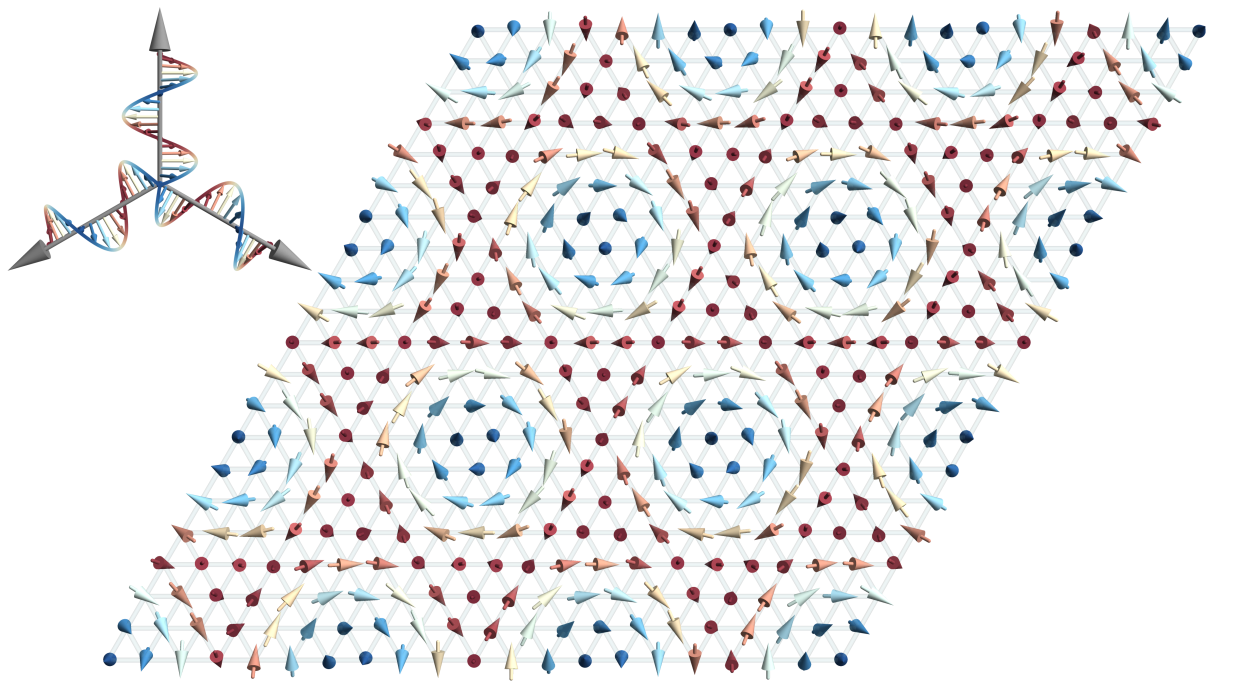
\includegraphics[width=\textwidth]{figure_01/skx_size20_theta3-20_shift0_mag_0+3Q_zero.png}
    \caption{\small {\bf Illustration of a multi-q state generating a skyrmion crystal.} Three helical spin waves with wave vectors summing up to zero in a two-dimensional plane, the initial phases at the origin are $\varphi_1=\varphi_2=\varphi_3=0$, generate a $3q$-skyrmion texture with $\vartheta=0.15$ on a triangular lattice.}
    \label{fig:3Qskx}
\end{figure}
}

%--------------------------
% Figure 2
%--------------------------

\newcommand{\figureII}{
\begin{figure*}[t!]
    \centering
    \begin{subfigure}[t]{0.5\textwidth}
        \centering
        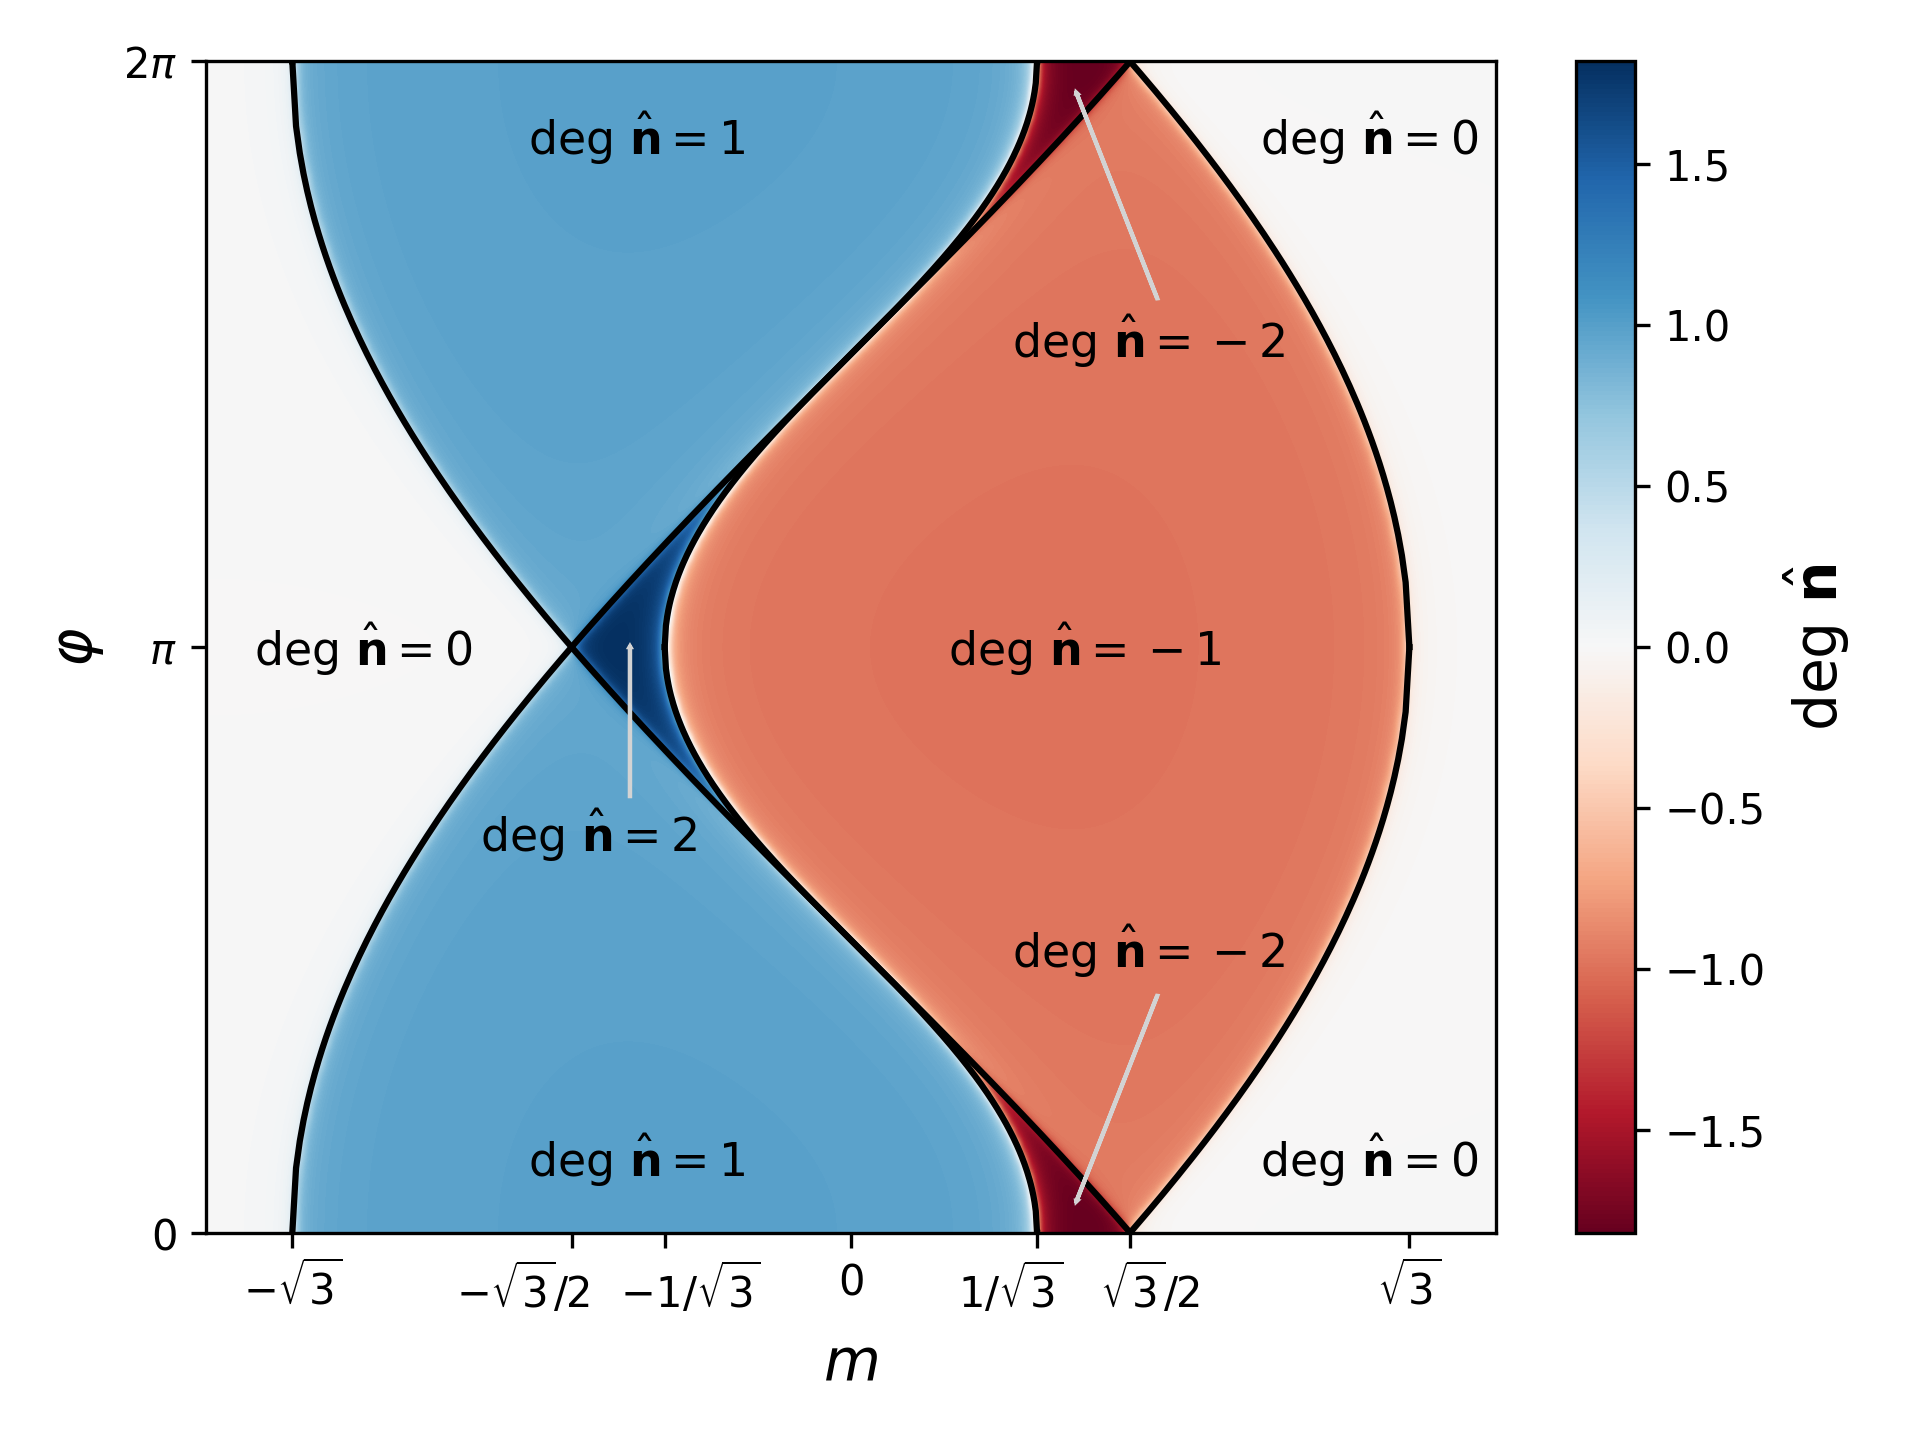
\includegraphics[width=\textwidth]{figure_02/plots/real_space_phase_diagram.png}
        \caption{\small Mapping degree}
    \end{subfigure}%
    ~ 
    \begin{subfigure}[t]{0.5\textwidth}
        \centering
        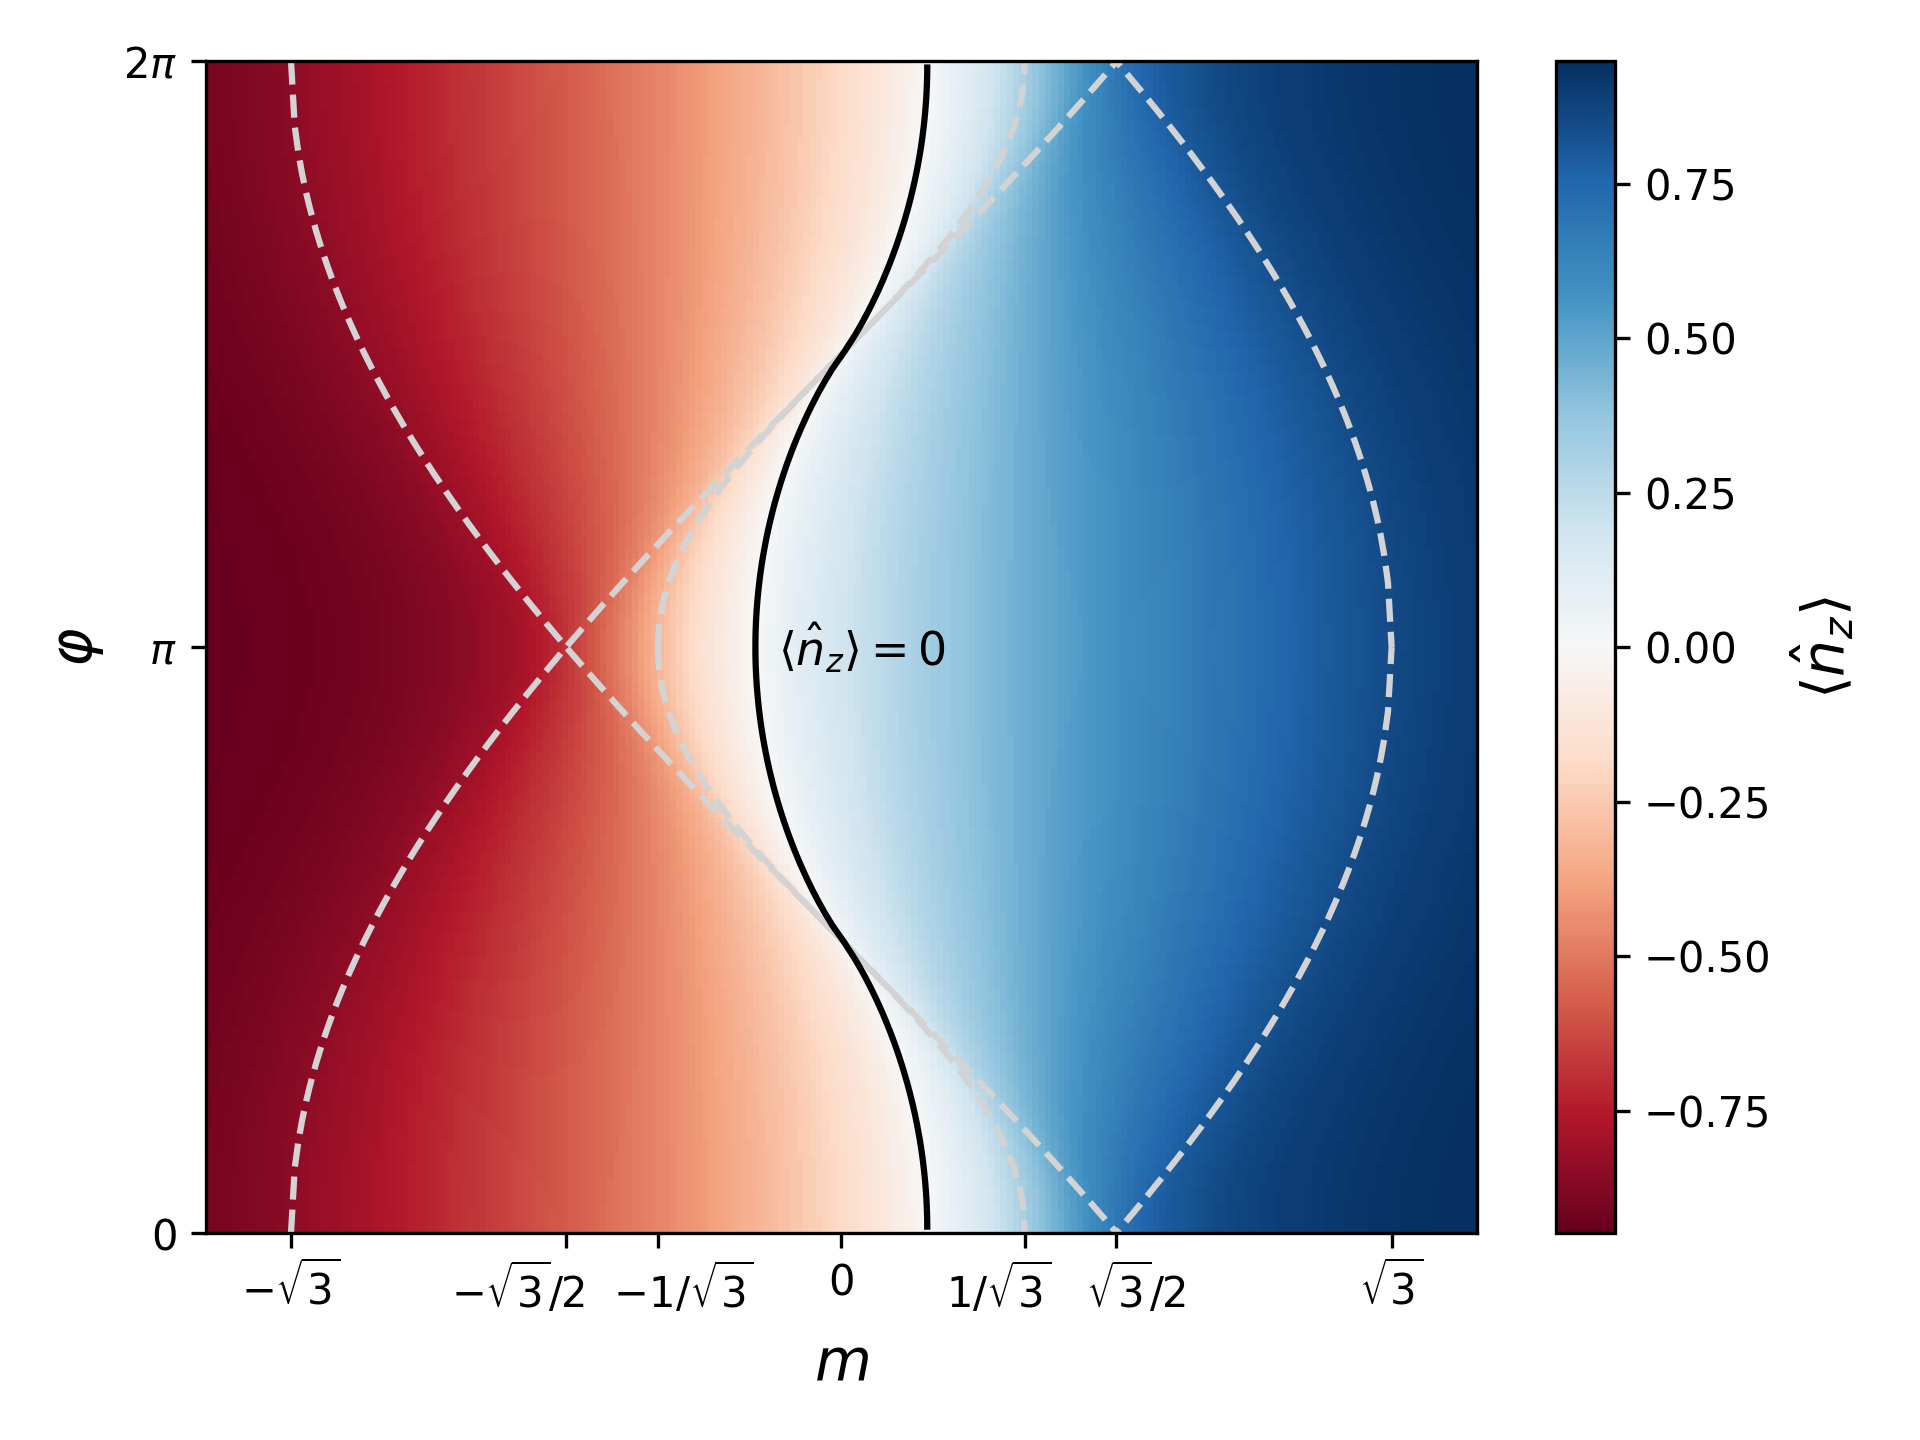
\includegraphics[width=\textwidth]{figure_02/plots/real_space_phase_diagram_nz.png}
        \caption{\small  Net magnetization}
    \end{subfigure}
    \caption{\small  {\bf Phase diagram of the $3\vec{q}$ skyrmion lattice.} The subfigures show order parameters of the magnetic texture as a function of $m$ and $\varphi$ which are relevant for the interpretation of the electronic structure. (a) Gives $\deg \hatn$, with  phase boundaries (solid black lines) determined by the condition that $\vec{n}(\vec{\varphi})=0$ for some $\vec{\varphi} \in T^2$ (cf. \cite[Fig. 6]{Shimizu2022}). (b) shows the net magnetization $\braket{\hat{n}_z}$ with phase boundary (solid black line) determined by the condition $\braket{\hat{n}_z}=0$.}
    \label{fig:3QskxPD}
\end{figure*}
}

% %--------------------------
% % Figure 3
% %--------------------------

\newcommand{\figureIIIa}{
\begin{figure}[t!]
     \centering
        \begin{subfigure}[t!]{\textwidth}
             \centering
             \caption{\small Density of states.}
             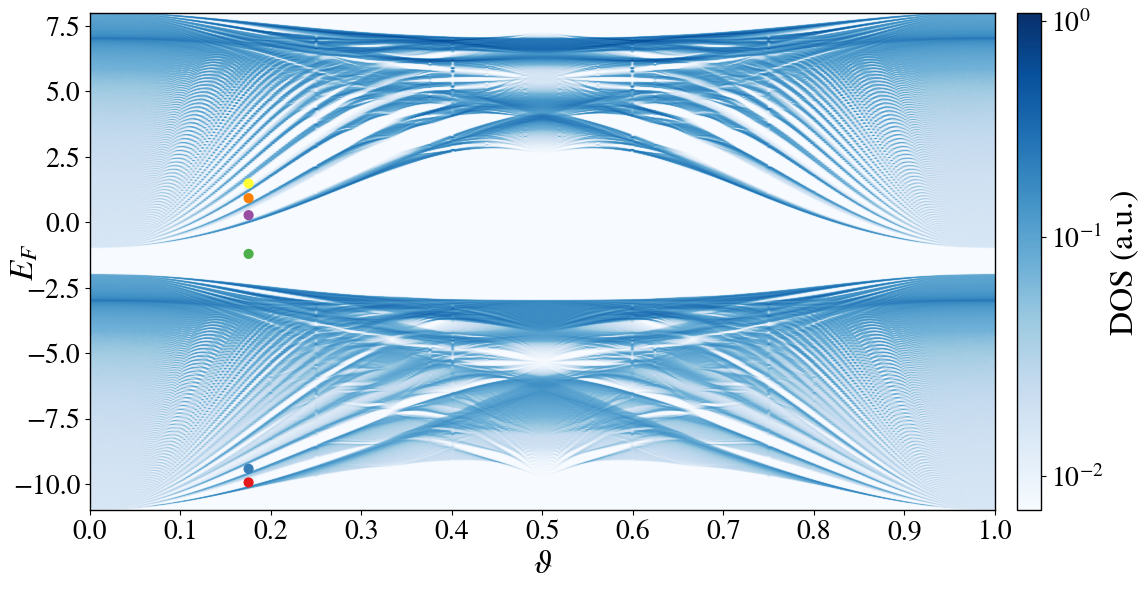
\includegraphics[width=\textwidth]{figure_03/plots/DoS_kpm_0shift0mag.png}
             \label{fig:DoS}
        \end{subfigure}
        \\
        \vspace{-5mm}
        \begin{subfigure}[t!]{0.9\textwidth}
            \centering
            \caption{\small Chern numbers at $\vartheta=\frac{10}{57}$.}
            \label{tab:ChernNum}
            \resizebox{\textwidth}{!}{\input{../gfx/figure_03/tables/ChernNumber_Table.txt}}
        \end{subfigure}
         \\
        \begin{subfigure}[t!]{\textwidth}
             \caption{\small Labels of $K$-theory class in $K_0(\mathcal{A})=\mathbb{Z}^8$.}
             \label{tab:ChernCoef}
             \centering
             \resizebox{\textwidth}{!}{\input{../gfx/figure_03/tables/ChernCoefficient_Table.txt}}
        \end{subfigure}
        \caption{\small {\bf Full topological classification of the 3$\vec{q}$ skyrmion crystal.} For the gaps labelled by the colored bullet points in the density of states (a), we compute all possible Chern numbers at $\vartheta=\frac{10}{57}$ in Table (b) and extract the corresponding $K$-theory class in Table (c). To a good accuracy, these values are given by integer numbers as expected. }
        \label{fig:Spectrum}
\end{figure}
}

% %--------------------------
% % Figure 4
% %--------------------------

\newcommand{\figureIVa}{
\begin{figure}[t!]
    \centering
    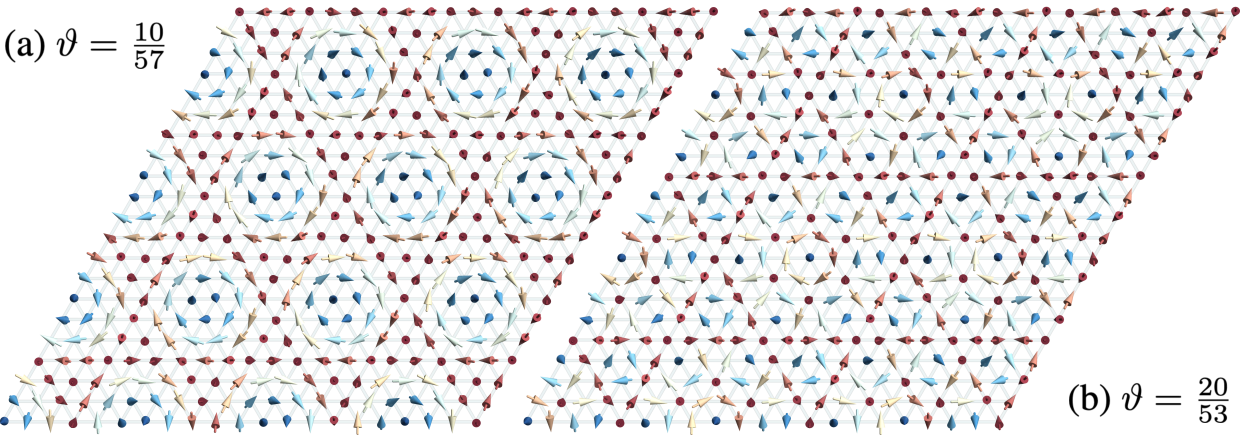
\includegraphics[width=\linewidth]{figure_04/skx_size20_theta10-57_20-53_shift0_mag_0.png}
    \caption{\small {\bf A skyrmionic multi-$q$ texture at $\vartheta=10/57$ and $\vartheta=20/53$}. The figure shows $20\times20$ parts of multi-$q$ textures with $\mathrm{deg}~\hatn=1$ ($\varphi=0$, $m=0$) for $\vartheta=10/57$ and for $\vartheta=20/53$ at which unusual band gap formations were noticed in the DOS plots of figure \ref{fig:ChernHierarchy}.
    While it is difficult to imagine that the texture in (b) still represents something like a skyrmion lattice, the electronic real-space winding number is indeed quantized.}
    \label{fig:skx_texture_scaling}
\end{figure}
}

% %--------------------------
% % Figure 5
% %--------------------------

\newcommand{\figureVa}{
\begin{figure}[t!]
    \centering
    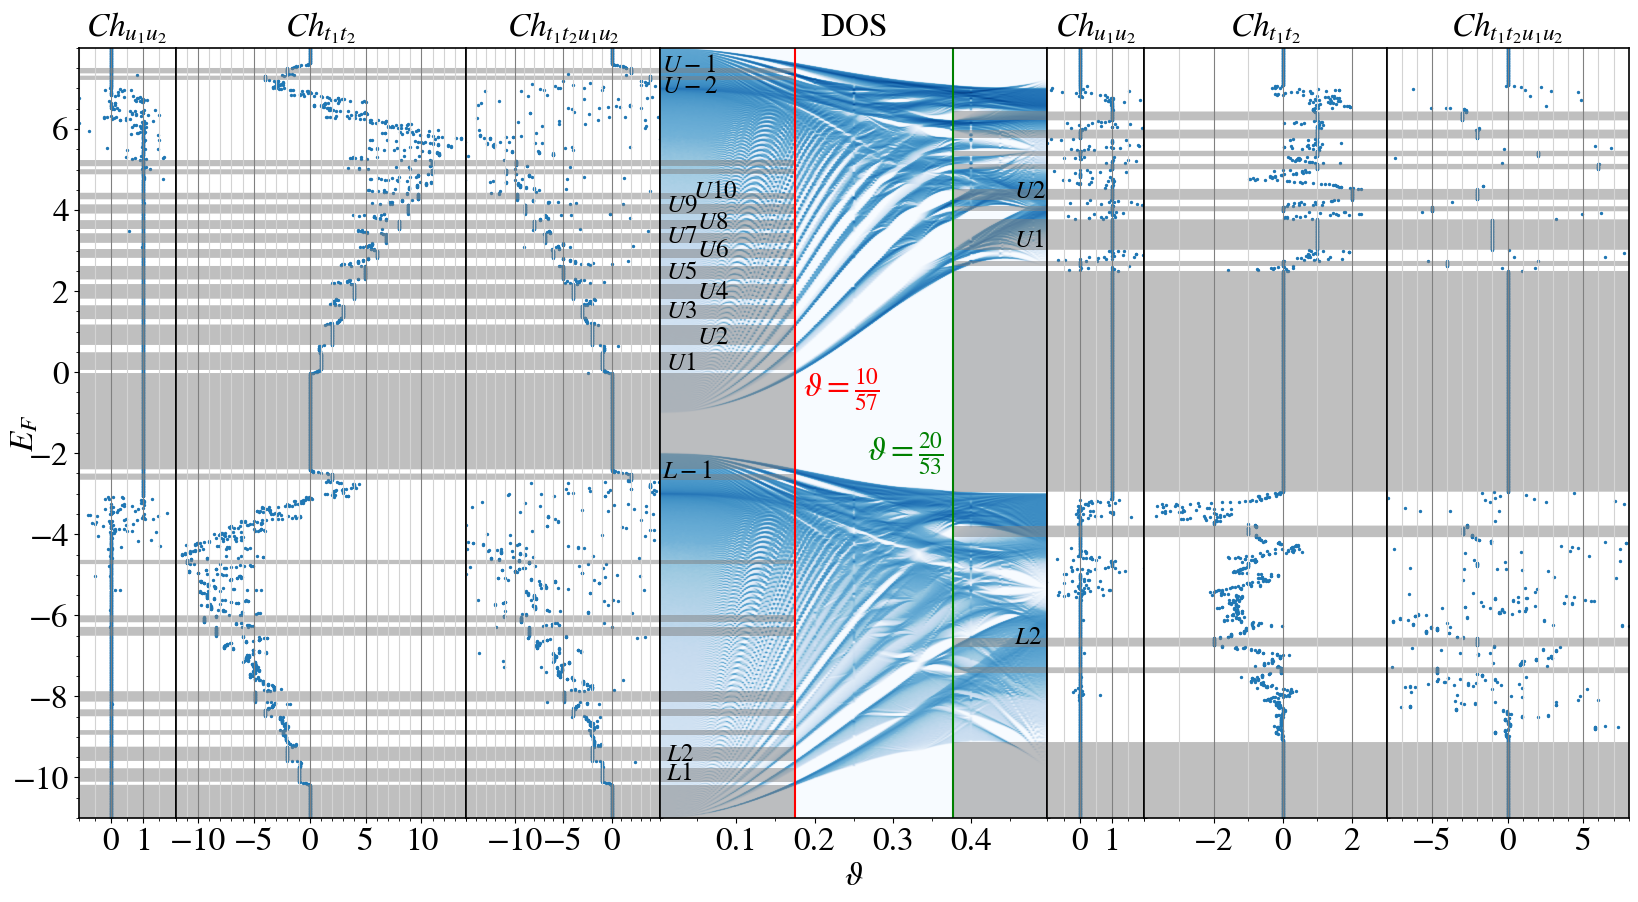
\includegraphics[width=1.0\linewidth]{figure_05/plots/Chernhierarchy_kpm_0shift0mag.png}
    \caption{\small {\bf Main Chern numbers of the skyrmion crystal at zero shift and magnetization.} At $\vartheta=\frac{10}{57}$ and $\vartheta=\frac{20}{53}$ we evaluate the Chern number in systems of size $57$ and $53$, respectively, for Fermi energies in the full energy range.}
    \label{fig:ChernHierarchy}
\end{figure}
}

% %--------------------------
% % Figure 6
% %--------------------------

\newcommand{\figureVIa}{
\begin{figure}[t!]
    \centering
    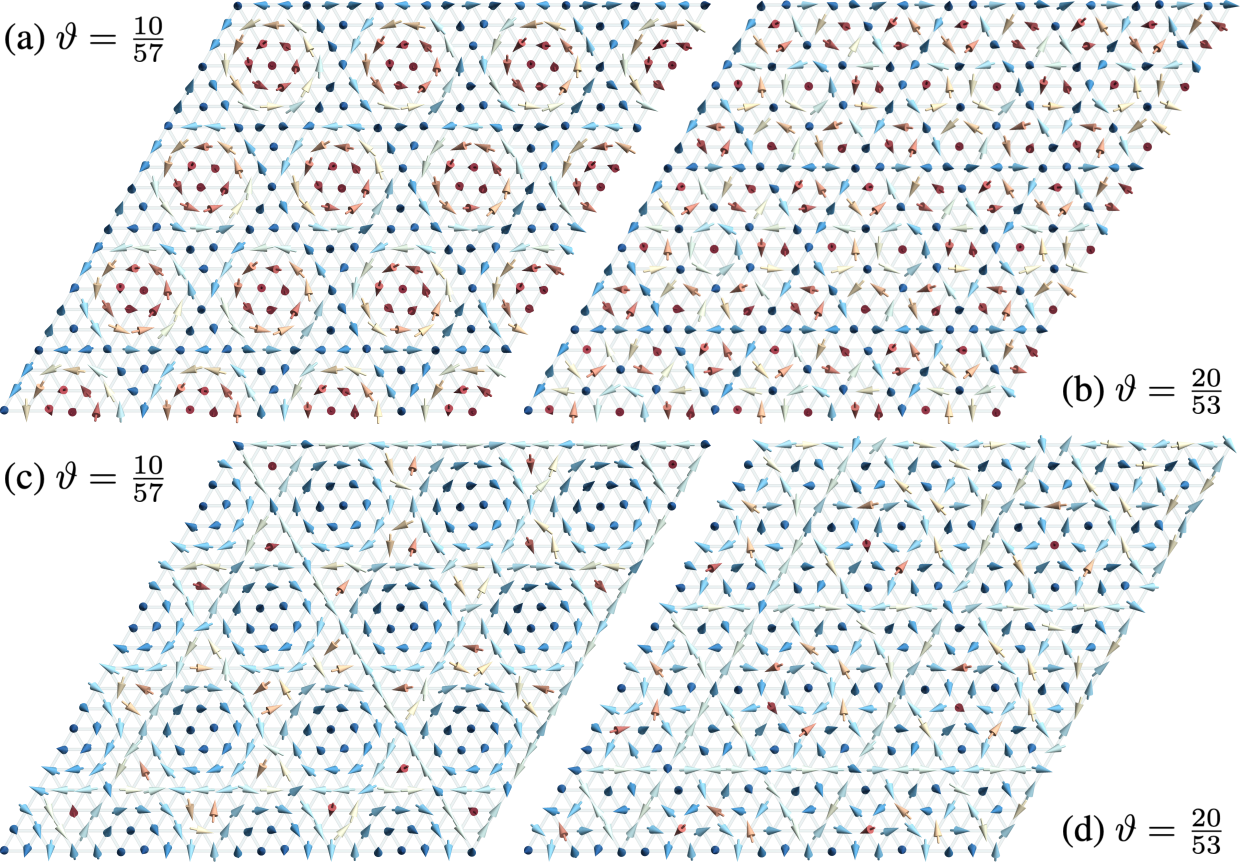
\includegraphics[width=\textwidth]{figure_06/skx_size20_theta10-57_20-53_shiftpi_mag_0__shift0_mag0dot7.png}
    \caption{\small {\bf Skyrmionic multi-$q$ textures for different parameters}. The figure shows $20\times20$ parts of multi-$q$ textures with $\mathrm{deg}~\hatn=-1$ ($\varphi=\pi$, $m=0$) in (a) and (b) and $\mathrm{deg}~\hatn=-2$ ($\varphi=0$, $m=0.7$) in (c) and (d) for $\vartheta=10/57$ and for $\vartheta=20/53$, respectively. The shift in $\varphi$ in (a) and (b) inverts the spin's directions and changes the relative position of the magnetic unit cell in comparison to fig. \ref{fig:skx_texture_scaling}.
    The magnetisation parameter $m$ raises the spins in $z$-direction. In (c) the winding $\mathrm{deg}~\hatn=-2$ is perceptible in the sharp corners of the rhombic magnetic unit cell.}
    \label{fig:skx_texture_phases}
\end{figure}
}

% %--------------------------
% % Figure 7
% %--------------------------

\newcommand{\figureVIIa}{
\begin{figure}[t!]
    \centering
    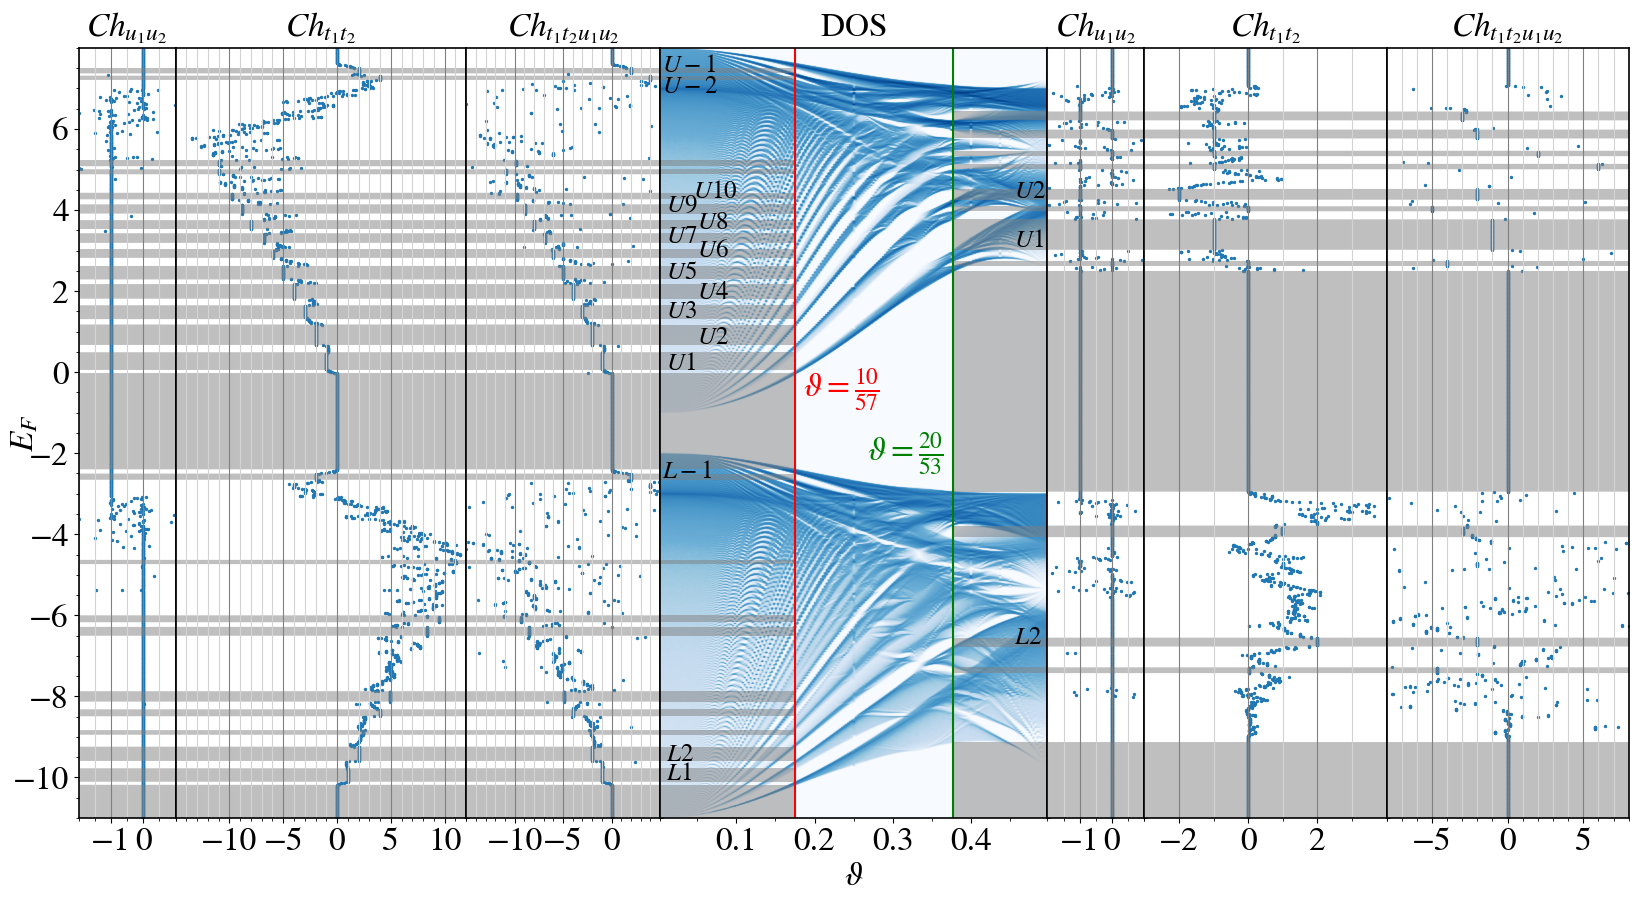
\includegraphics[width=1.0\linewidth]{figure_07/plots/Chernhierarchy_kpm_pishift0mag.png}
    \caption{\small {\bf Main Chern numbers of the skyrmion crystal at $\pi$ shift and zero magnetization.} At $\vartheta=\frac{10}{57}$ and $\vartheta=\frac{20}{53}$, we evaluate the Chern number in systems of size $57$ and $53$, respectively, for Fermi energies in the full energy range.}
    \label{fig:ChernHierarchyShift}
\end{figure}
}

% %--------------------------
% % Figure 8
% %--------------------------

\newcommand{\figureVIIIa}{
\begin{figure}[t!]
    \centering
    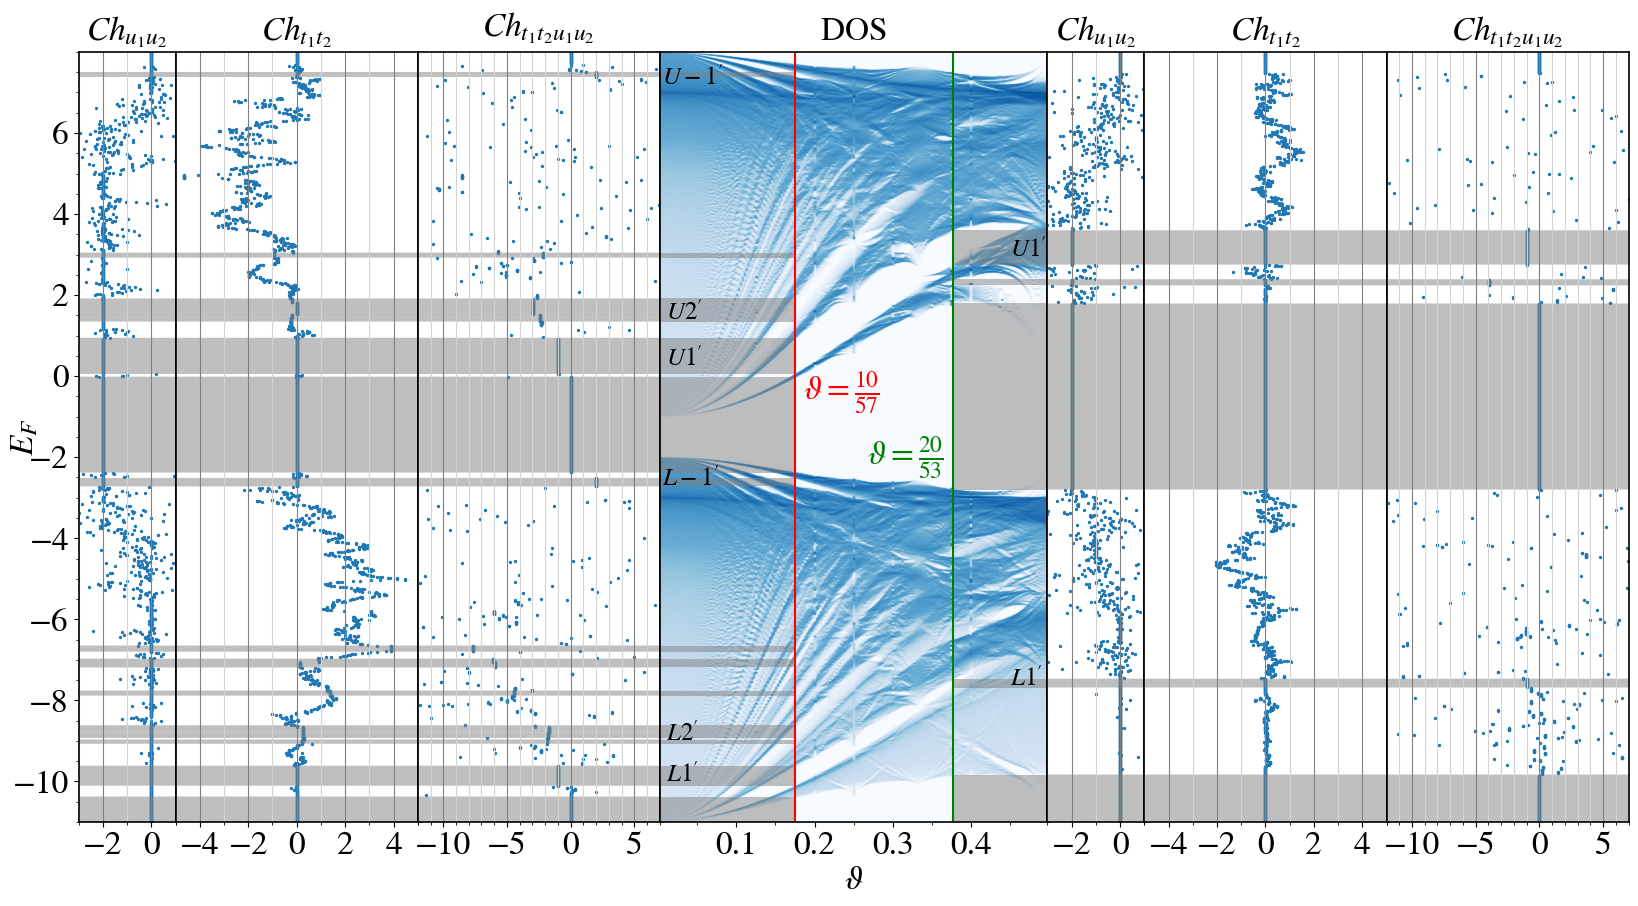
\includegraphics[width=1.0\linewidth]{figure_08/plots/Chernhierarchy_kpm_0shift07mag.png}
    \caption{\small {\bf Main Chern numbers of the skyrmion crystal at zero shift and $0.7$ magnetisation.} At $\vartheta=\frac{10}{57}$ and $\vartheta=\frac{20}{53}$ we evaluate the Chern number in systems of size $57$ and $53$, respectively, for Fermi energies in the full energy range.}
    \label{fig:ChernHierarchyMag}
\end{figure}
}

% %--------------------------
% % Figure 9
% %--------------------------

\newcommand{\figureIXa}{
\begin{figure}[t!]
    \centering
    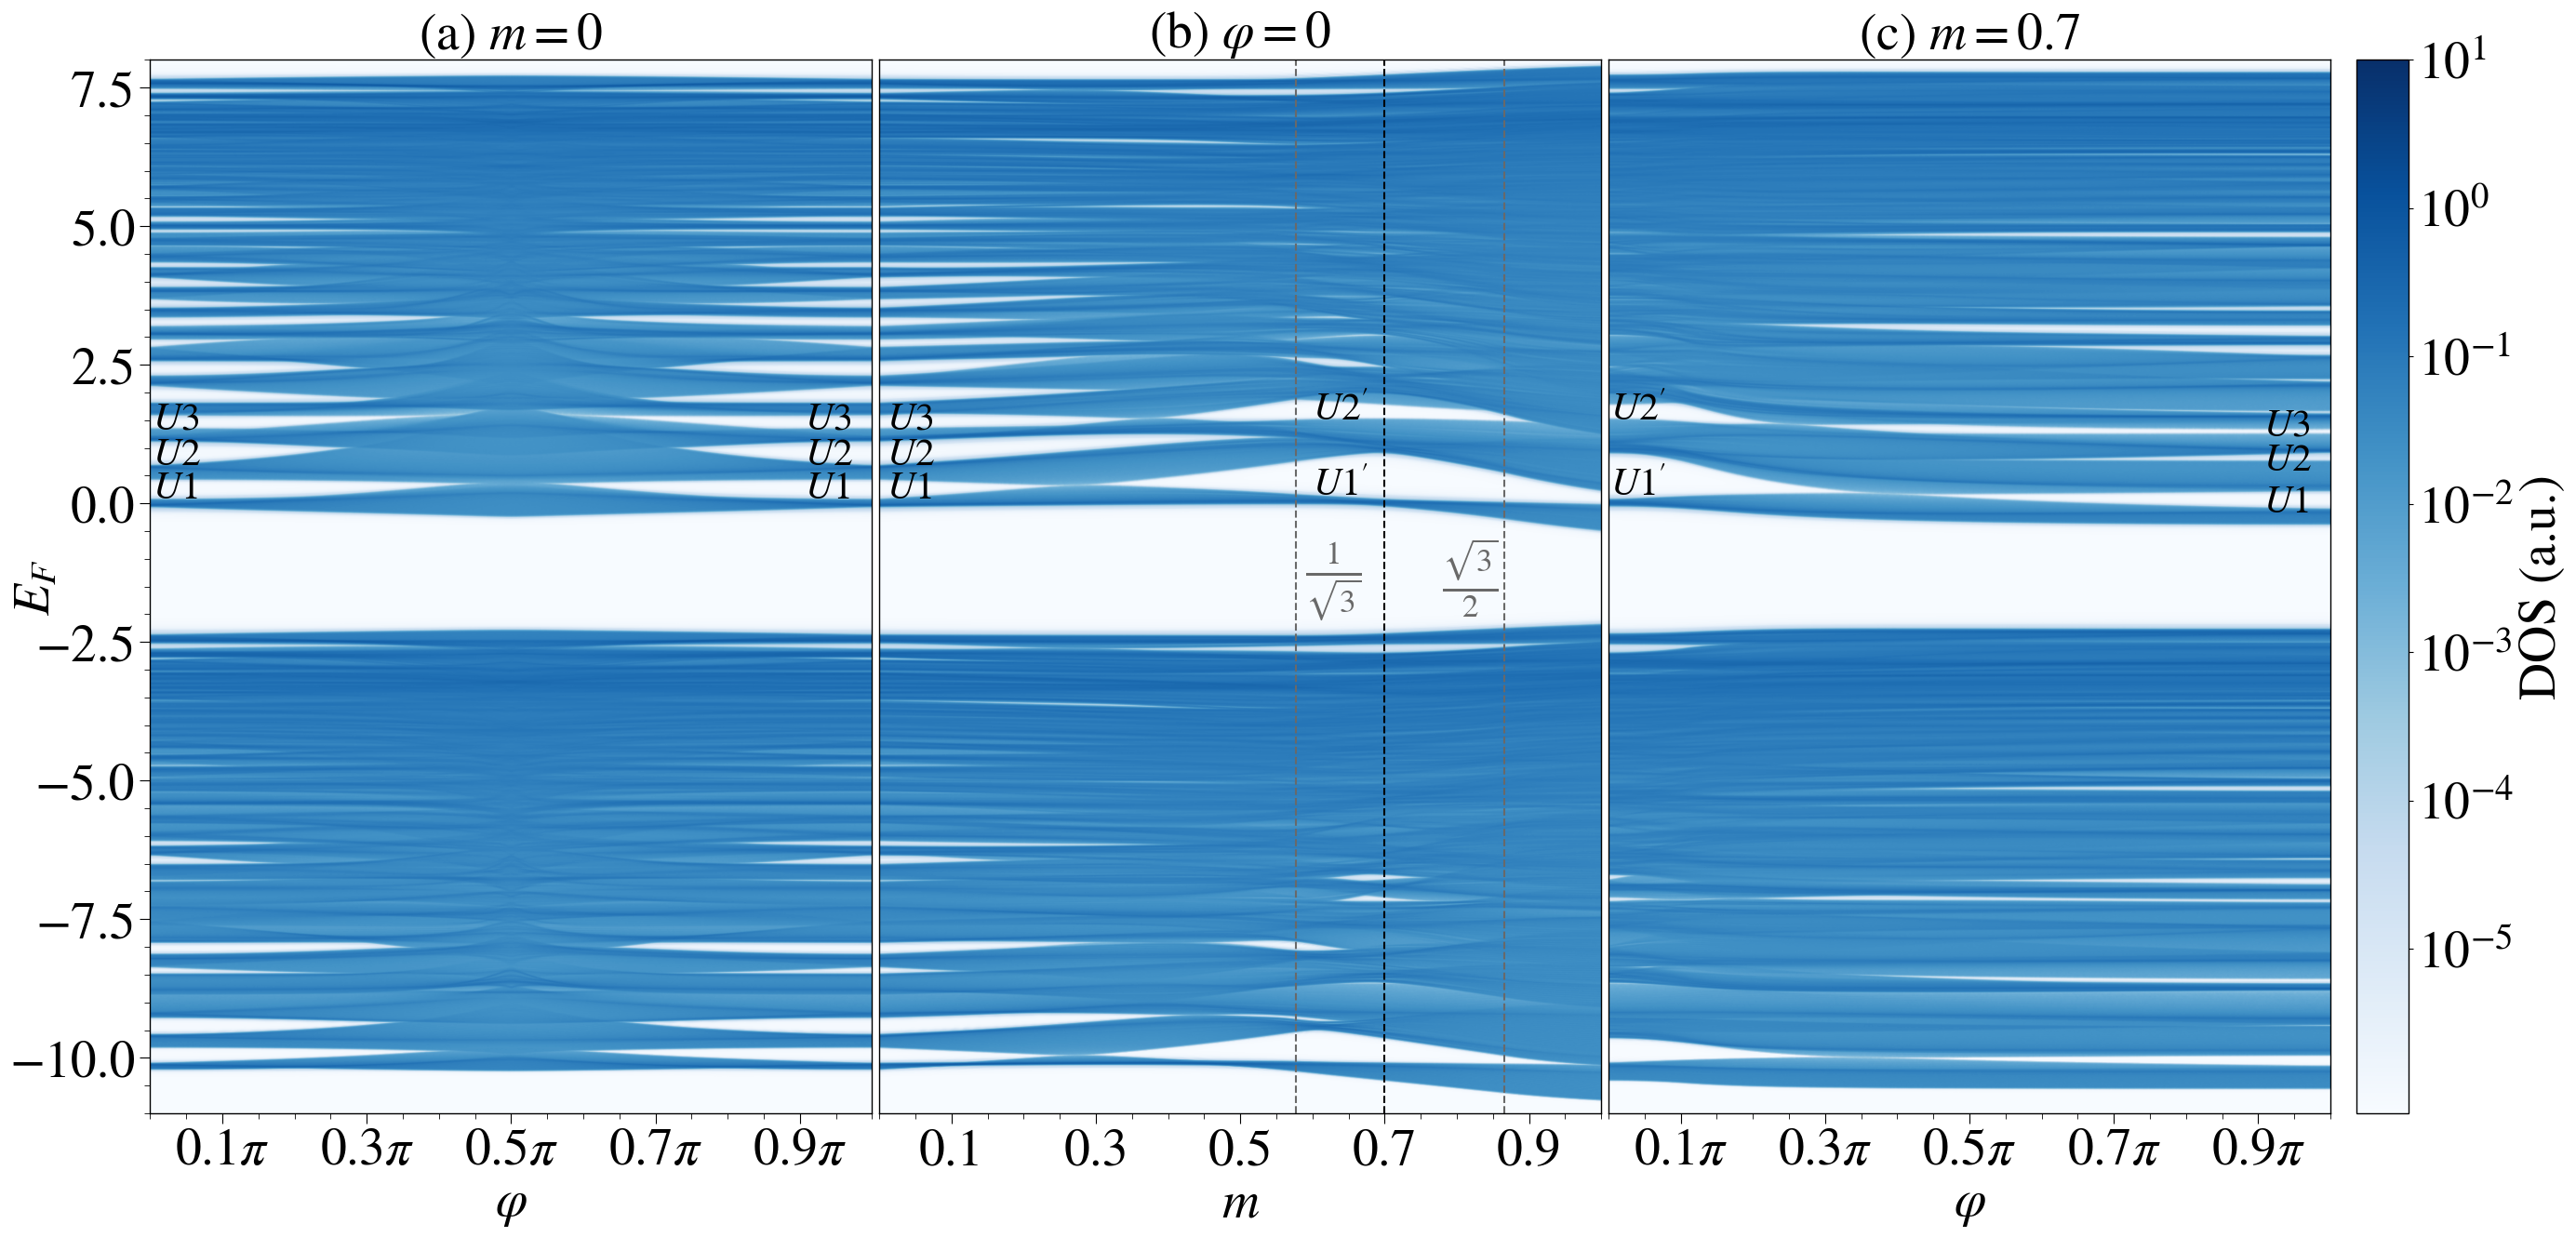
\includegraphics[width=\textwidth]{figure_09/plots/DoS_transitions.png}
    \caption{\small {\bf Density of states evolution across real-space phase transitions.} We perform three different line cuts through the phase space spanned by the texture parameters $(m,\varphi)$.}
    \label{fig:DoSShifts}
\end{figure}
}

% %--------------------------
% % Figure 10
% %--------------------------

\newcommand{\figureXa}{
\begin{figure}[t!]
     \centering
        \begin{subfigure}[t!]{0.32\textwidth}
             \centering
             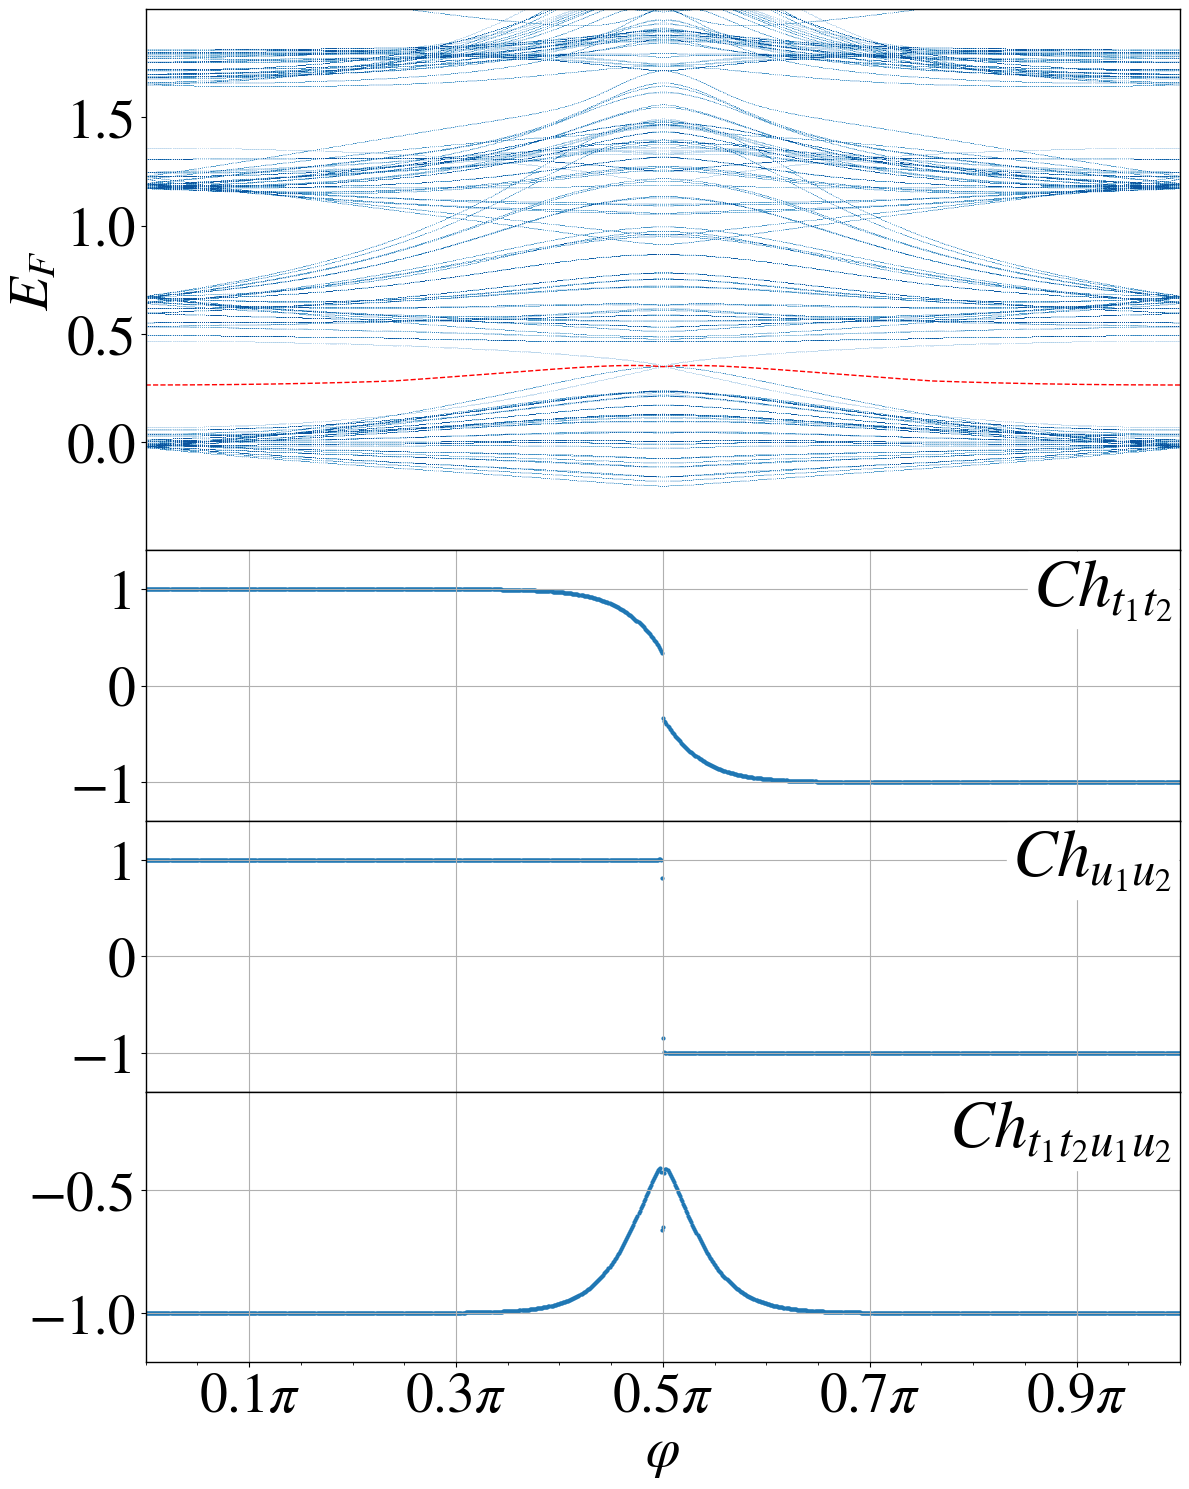
\includegraphics[width=\textwidth]{figure_10/plots/Chernhierarchy_phaseshift_0mag.png}
             \caption{\small $m=0$}
             \label{fig:Chernshift0mag}
        \end{subfigure}
        \begin{subfigure}[t!]{0.32\textwidth}
             \centering
             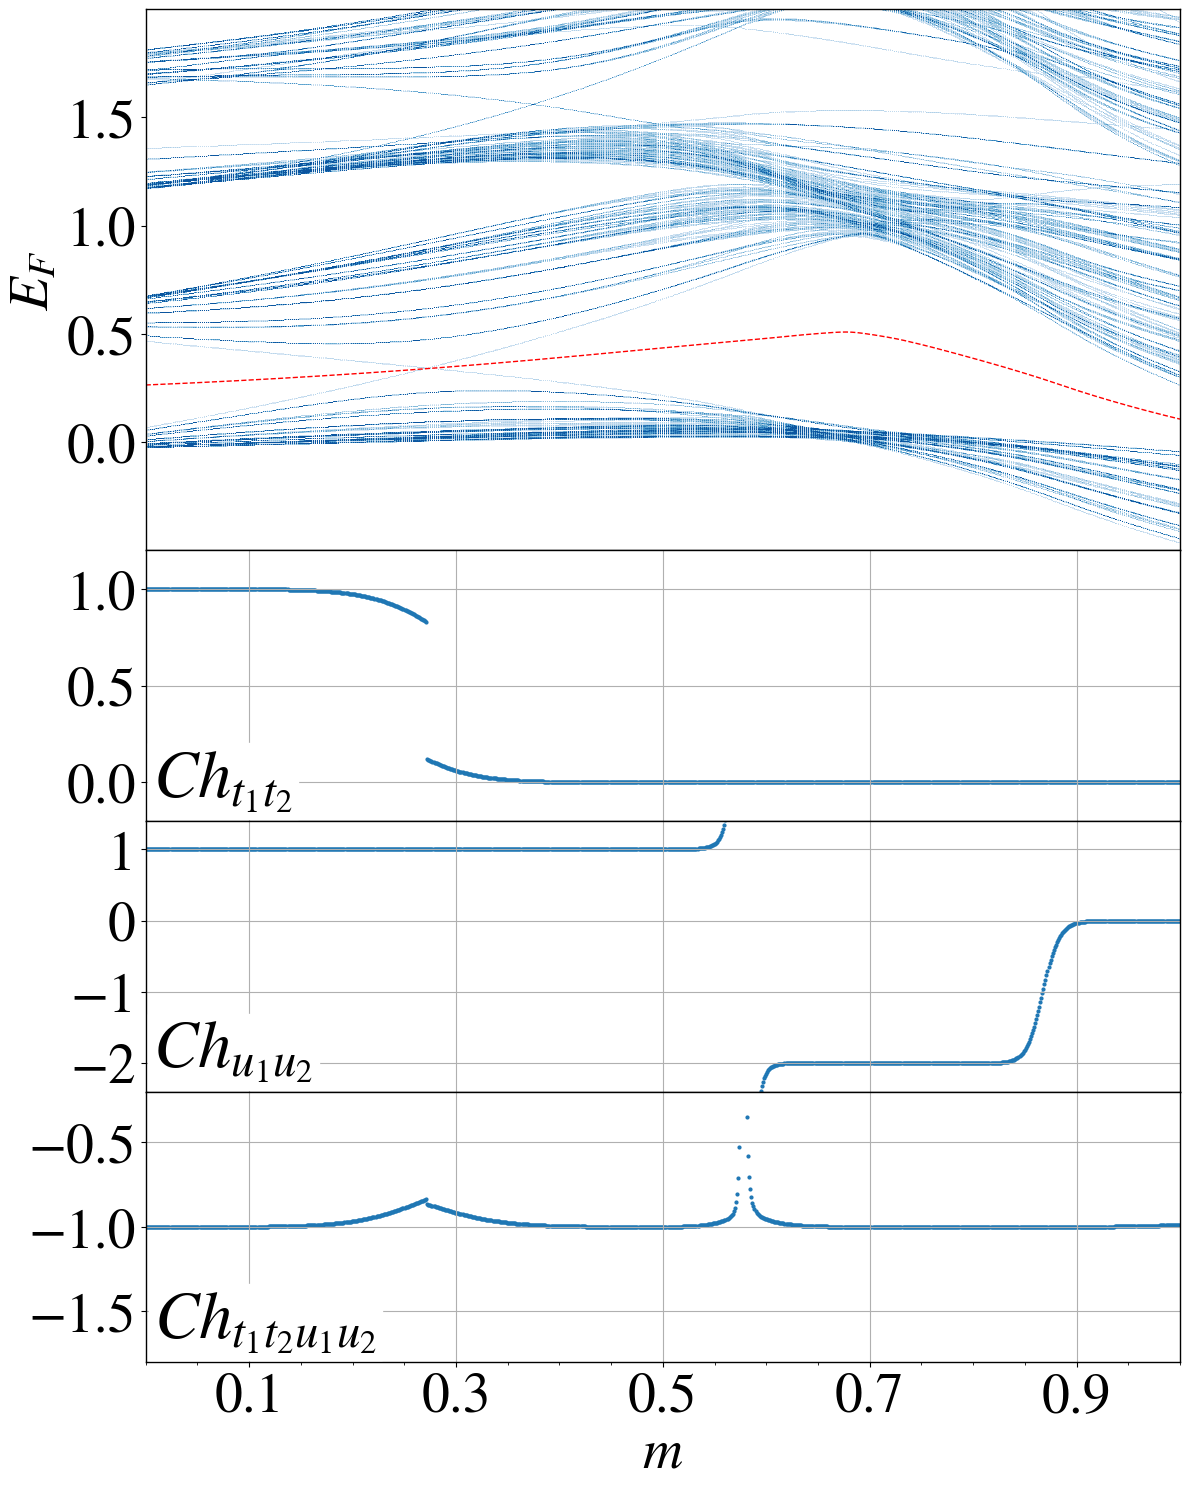
\includegraphics[width=\textwidth]{figure_10/plots/Chernhierarchy_magnetisation_0shift.png}
             \caption{\small $\varphi=0$}
             \label{fig:Chernmag0shift}
        \end{subfigure}
        \begin{subfigure}[t!]{0.32\textwidth}
            \centering
            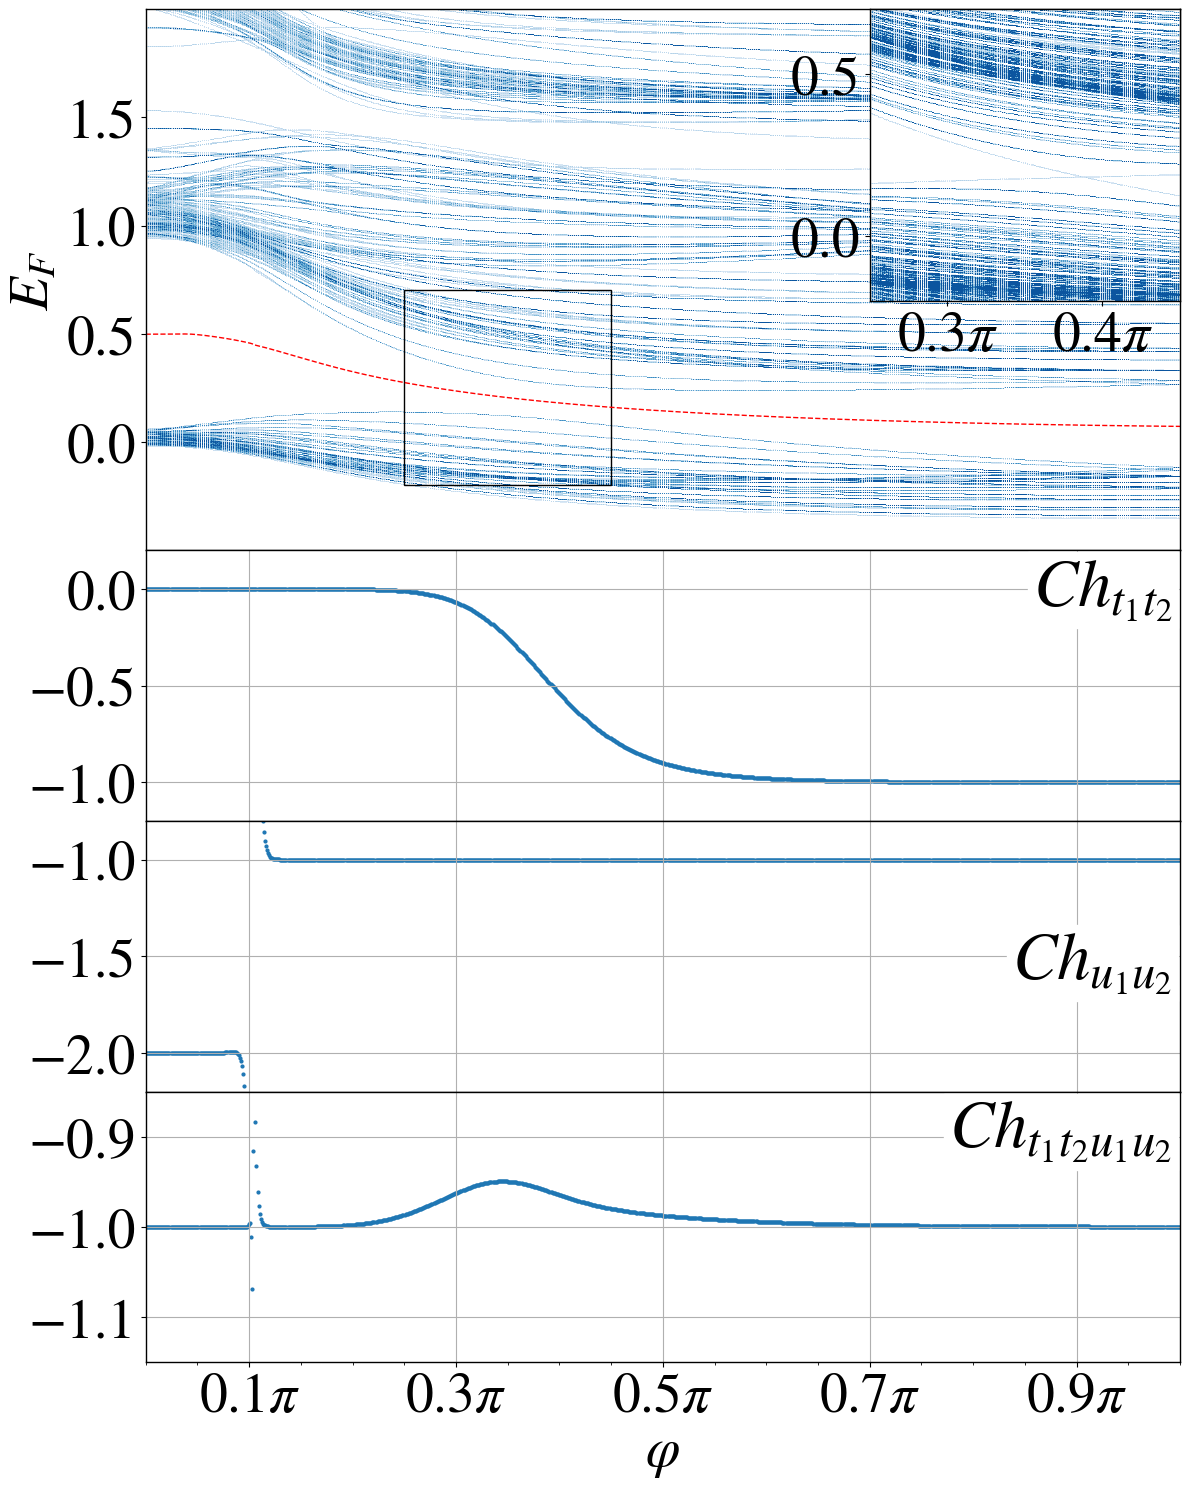
\includegraphics[width=\textwidth]{figure_10/plots/Chernhierarchy_phaseshift_07mag_inset.png}
            \caption{\small $m=0.7$}
            \label{fig:Chernshift07mag}
        \end{subfigure}
        \caption{\small {\bf Chern number evolution across real-space phase transitions.}
        We perform three line cuts through the phase space spanned by the texture parameters $(m,\varphi)$.
        We compute the main Chern numbers of the first gap by fixing the IDS to $1+1\cdot\left( \frac{10}{57} \right)^2$ in a system with $57\times57$ sites and $\vartheta=\frac{10}{57}$, the red dashed line marks the Fermi energy positioned in the middle of the gap.
        The inset in subfigure (c) displays the energy eigenvalues computed in a larger system with $137 \times 137$ sites and $\vartheta=\frac{24}{137}$.}
        \label{fig:ChernShifts}
\end{figure}
}

% %--------------------------
% % Figure 11
% %--------------------------

\newcommand{\figureXIa}{
\begin{figure}[t!]
    \centering
    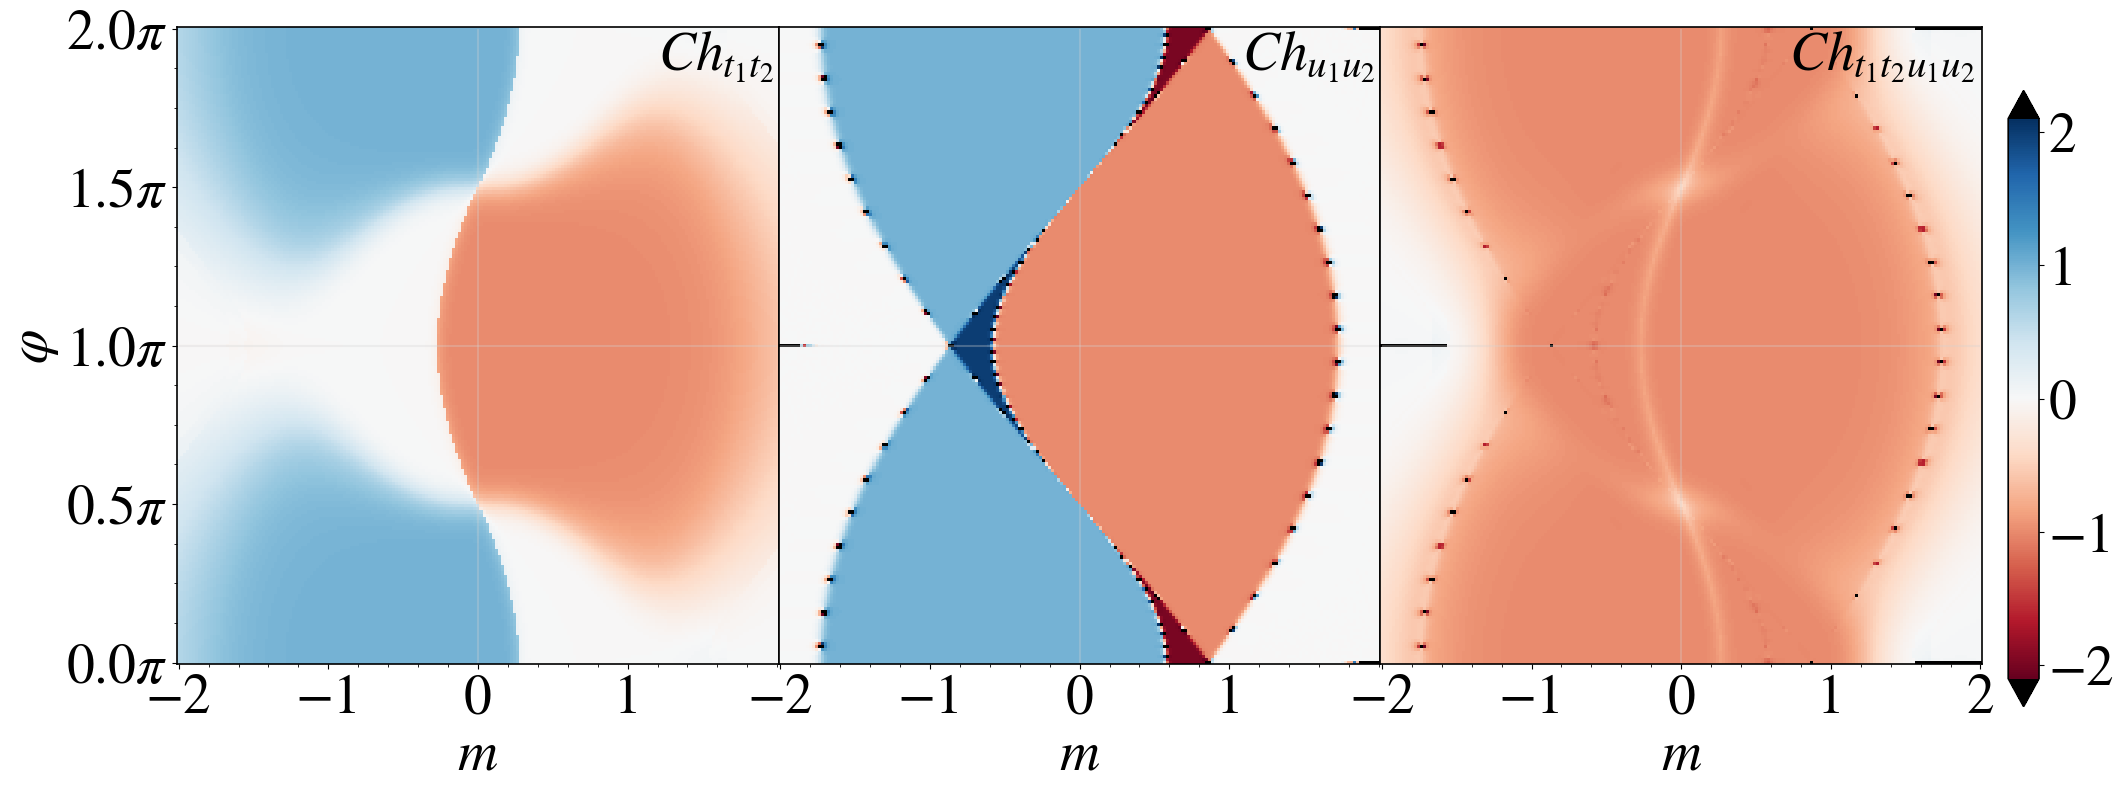
\includegraphics[width=1.0\linewidth]{figure_11/plots/ChernDiagram3.png}
    \caption{\small {\bf Topological phase diagrams.} For  constant $\mathrm{IDS}=1+1\cdot\left( \frac{10}{57} \right)^2$, these figures trace the Chern numbers across the phase space spanned by $(m, \varphi)$. Notably, $\mathrm{Ch}_{u_1 u_2}$ is in one-to-one correspondence with the phase diagram obtained through $\deg\hatn$ of the texture.
    $\mathrm{Ch}_{t_1 t_2}$ has a pronounced correlation with the net-magnetization of the real-space texture, while $\mathrm{Ch}_{t_1 t_2 u_1 u_2}$ seems to be responsive to both of these qualities of the real-space texture.}
    \label{fig:ChernDiagram}
\end{figure}
}

% %--------------------------
% % Figure 12
% %--------------------------

\newcommand{\figureXIIa}{
\begin{figure}[t!]
    \centering
    \centering
    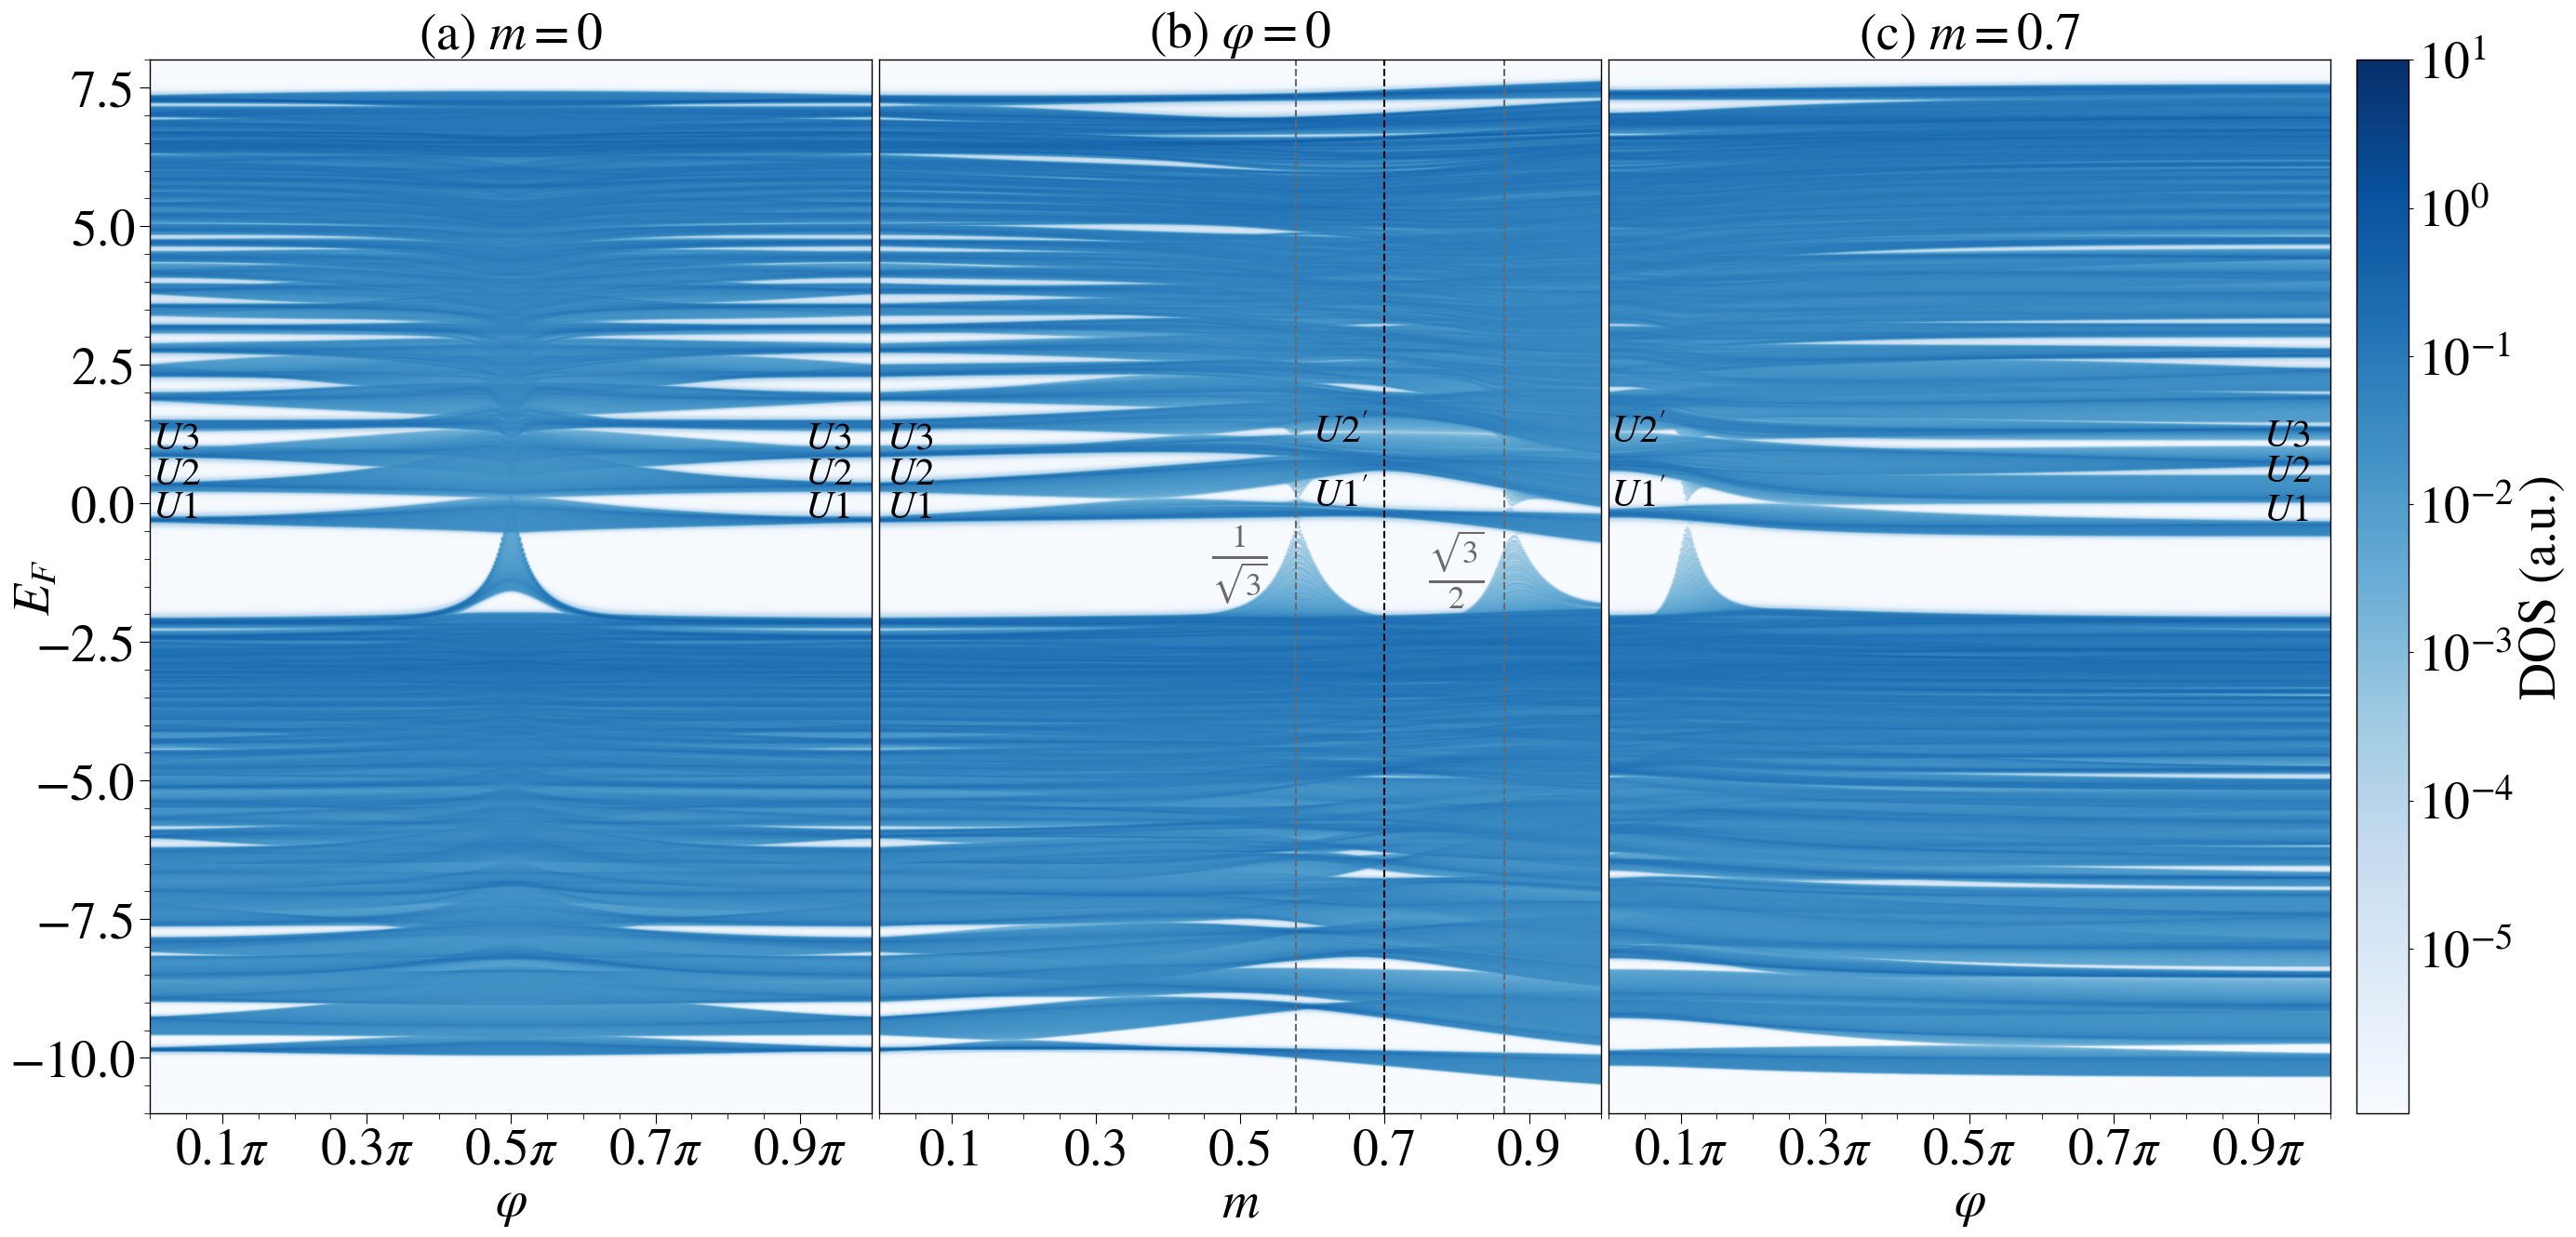
\includegraphics[width=\textwidth]{figure_12/plots/DoS_transitions_reg01.png}
        \caption{\small {\bf Density of states evolution across real-space phase transitions with regularization.} We perform three different line cuts through the phase space spanned by the texture parameters $(m,\varphi)$. The texture is regularized with $\eta=0.1$.}
        \label{fig:DoSShiftsReg}
\end{figure}
}

% %--------------------------
% % Figure 13
% %--------------------------

\newcommand{\figureXIII}{
\begin{figure}[t!]
     \centering
         \begin{subfigure}[t!]{0.32\textwidth}
             \centering
             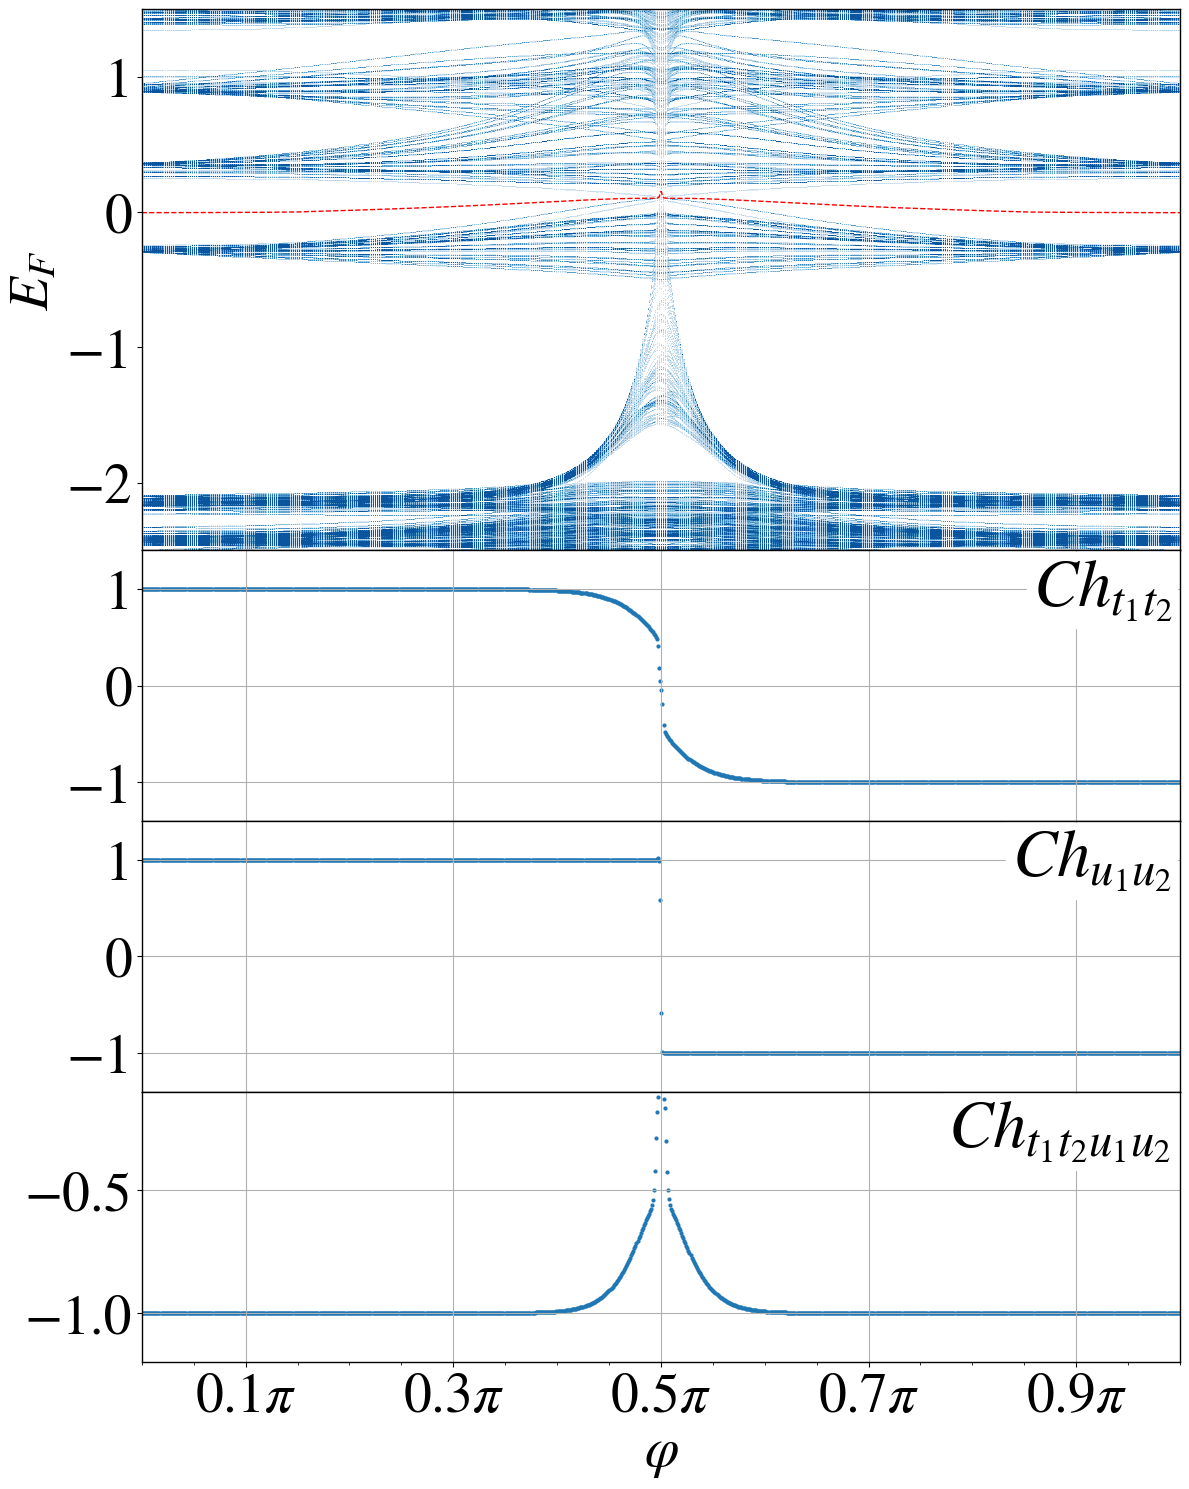
\includegraphics[width=\textwidth]{figure_13/plots/Chernhierarchy_phaseshift_0mag_reg01.png}
             \caption{\small $m=0$}
             \label{fig:Chernshift0magReg}
         \end{subfigure}
         \begin{subfigure}[t!]{0.32\textwidth}
             \centering
             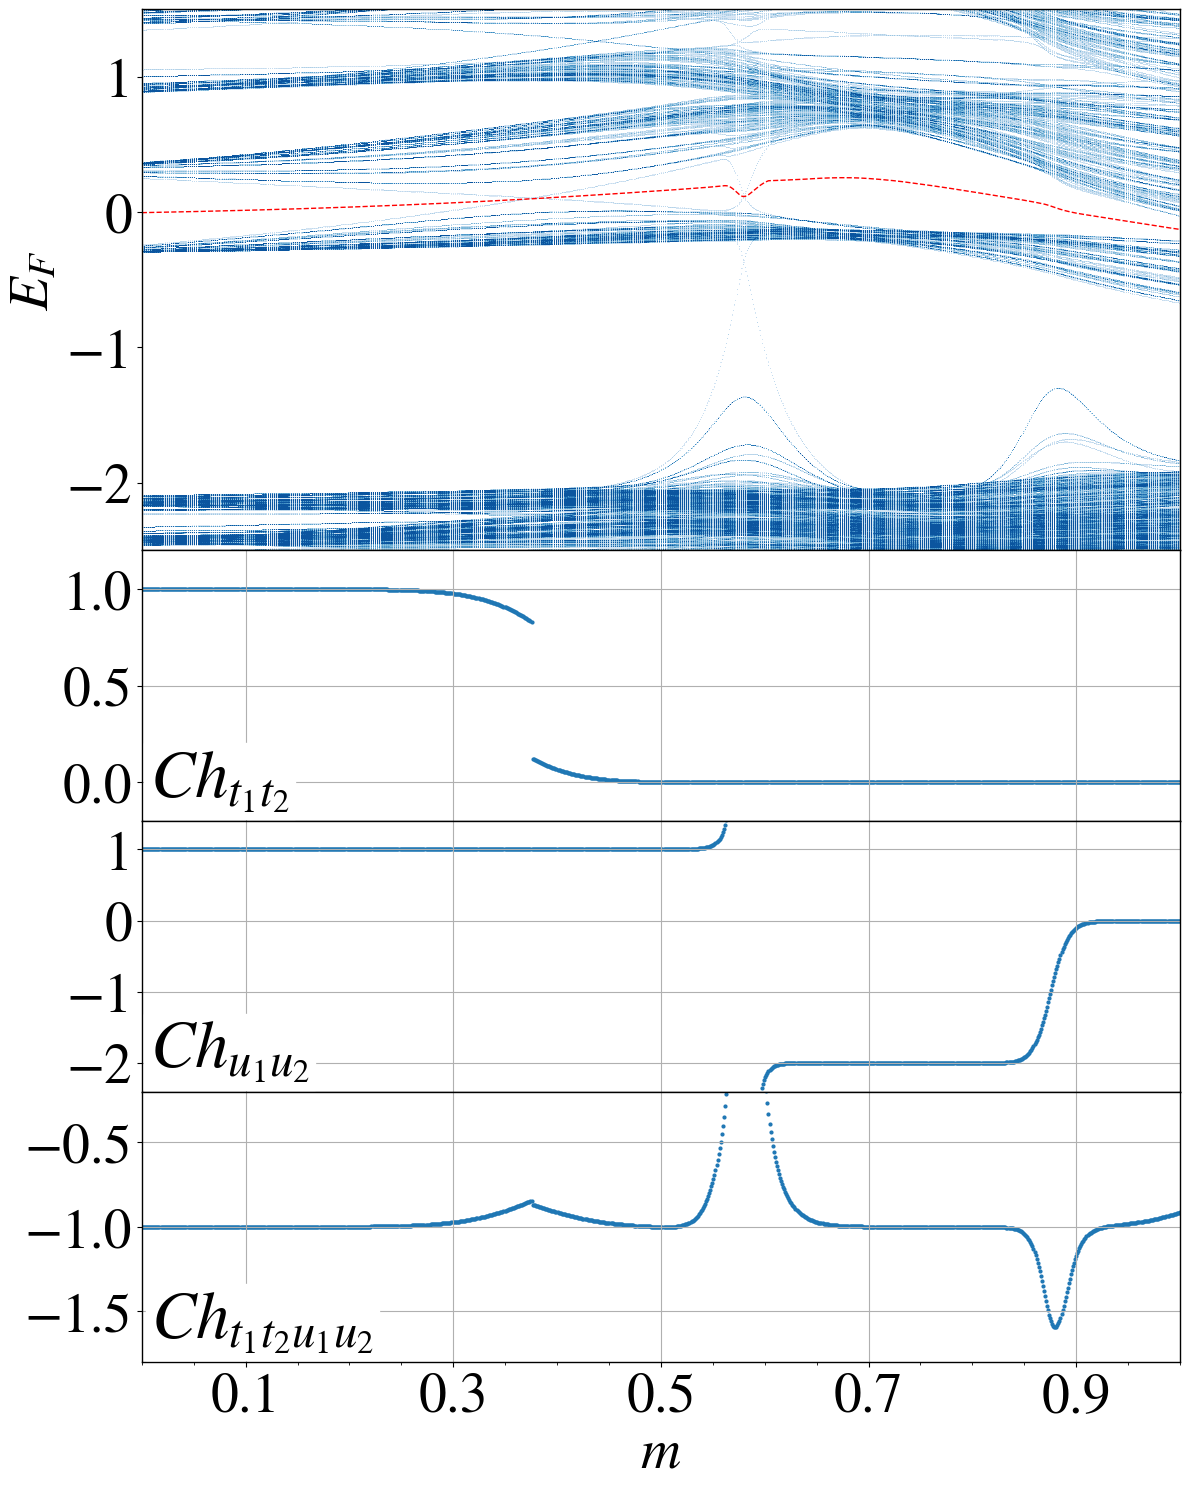
\includegraphics[width=\textwidth]{figure_13/plots/Chernhierarchy_magnetisation_0shift_reg01.png}
             \caption{\small $\varphi=0$}
             \label{fig:Chernmag0shiftReg}
         \end{subfigure}
         \begin{subfigure}[t!]{0.32\textwidth}
            \centering
            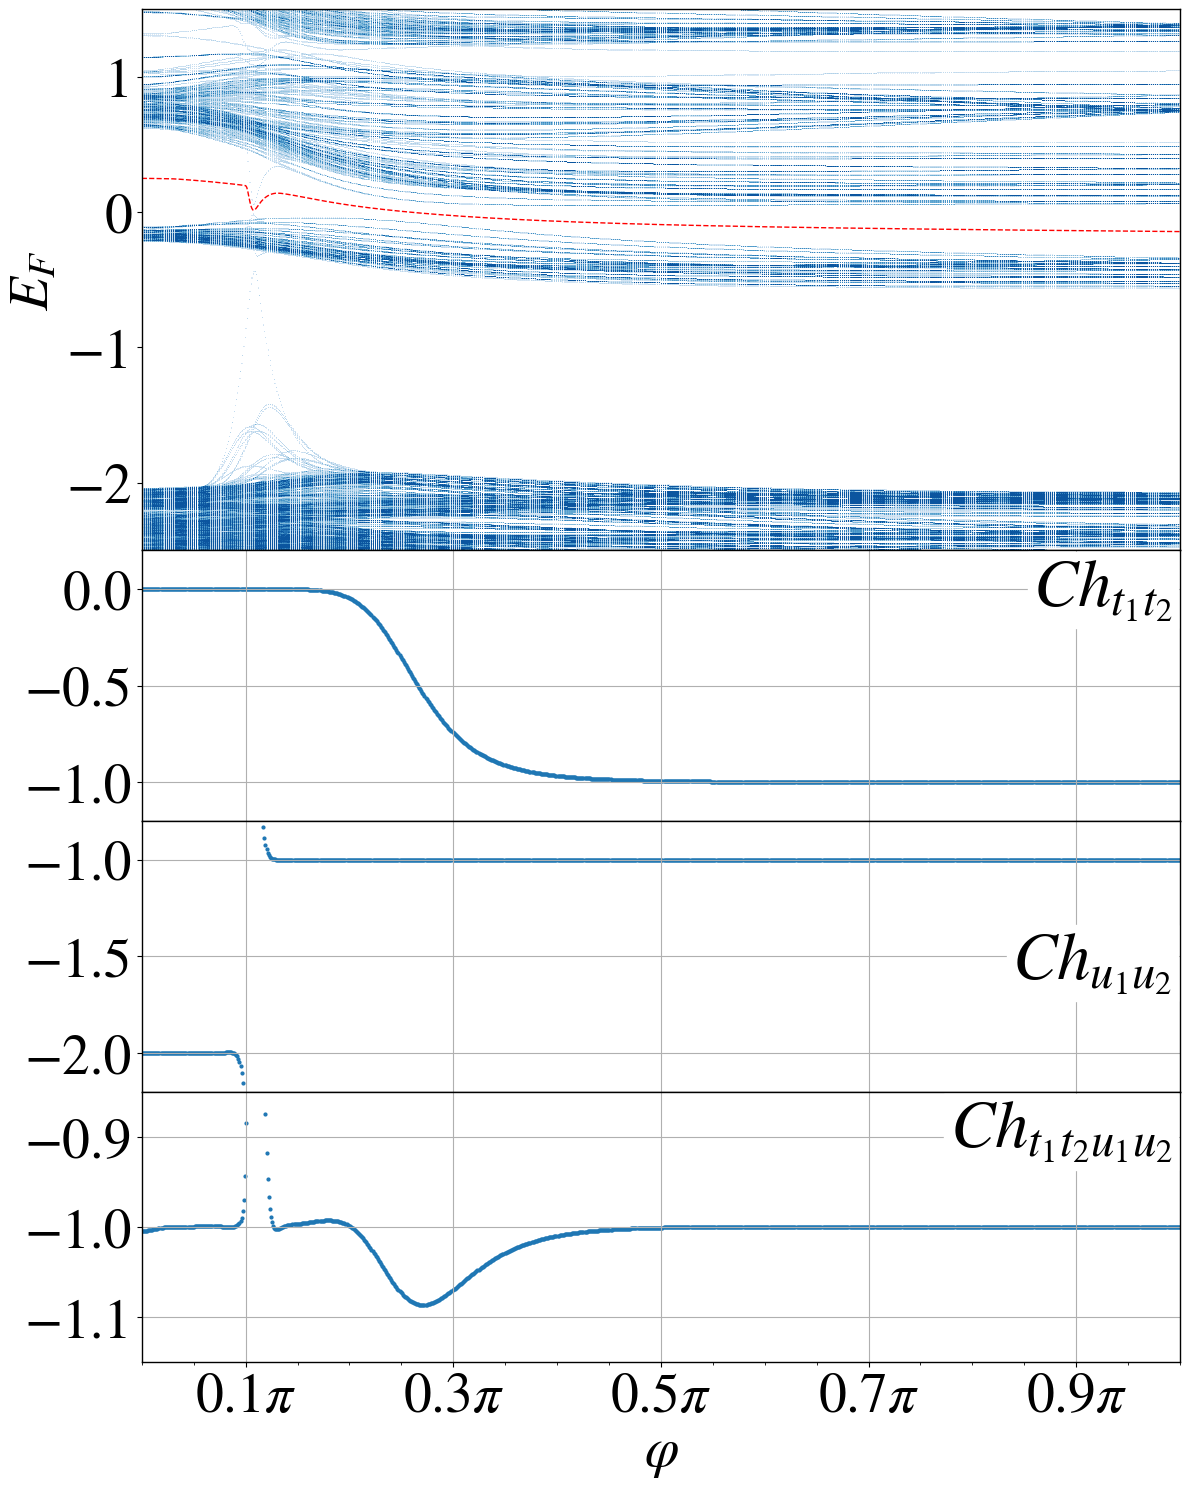
\includegraphics[width=\textwidth]{figure_13/plots/Chernhierarchy_phaseshift_07mag_reg01.png}
            \caption{\small $m=0.7$}
            \label{fig:Chernshift07magReg}
         \end{subfigure}
        \caption{\small {\bf Chern number evolution across real-space phase transitions with regularization.} We perform three different line cuts through the phase space spanned by the texture parameters $(m,\varphi)$. We compute the main Chern numbers of the first gap by fixing the IDS to $1+1\cdot\left( \frac{10}{57} \right)^2$ in a system with $57\times57$ sites and $\vartheta=\frac{10}{57}$, the red dashed line marks the Fermi energy positioned in the middle of the gap.}
        \label{fig:ChernShiftsReg}
\end{figure}
}